\chapter{Block Rewards and Selfish Mining}


\section{What we see in this chapter}
Chapter 10 marks rather
an interesting turning point for us
in this course because
thus far, we've been focused
entirely on the problem of consensus
which of course is the
fundamental problem that pretty much any
blockchain protocol must solve it and must
keep a bunch of computers in sync so
they all agree on the state of the
blockchain. So, accordingly, we've been
studying lots of protocols and
possibility results
thinking about consistent thinking
about liveness, and looking at
different models of the communication
Network and then even in Chapter 9 we started talking about
permissionless consensus, civil
resistance, proof of work, but it's 
all been about consensus all the time. There are 
two things that
we now are wondering about:\\
\begin{itemize}
  \item The first thing we might be wondering about or started wondering after chapter 9,
when we started talking about proof of
work and those running a protocol and working hard to try to solve these
hard crypto puzzles, we
haven't talked out all about incentives.
So why would any node bother to run
run of these consensus protocols. For example, if you're IBM in the 1980s and
you're just buying seven servers to replicate a database for high uptime,
who cares you don't need to worry about
incentives; the company just buys
the seven servers and runs it, end of
story! However, in a permissionless context
where basically nodes can just
start running the protocol
whenever they want especially if running
the protocol involves doing all
this hashing and looking for
solutions to hard crypto puzzles, what
would motivate a node to bother
to join the party and run your 
consensus protocol?
  \item The second thing is that
we've now had nine chapters but, we haven't
talked about
cryptocurrencies at all
and some of you maybe are wondering that
aren't cryptocurrencies the entire point
of a blockchain protocol? The answer
to that question is not right. So,
it's true that the story of
cryptocurrencies and the story of
blockchain protocols have been very
intertwined up to this point and that
may well continue to be true for some
time but as the last many
chapters have shown, you can have a
blockchain protocol without having a
cryptocurrency
and this chapter will be the first one
where we're not talking
about blockchain protocols completely
abstractly, but specifically the
protocols that host a cryptocurrency
that have some currency native to the
protocol.
So what do I mean by a native currency?
Well, I just mean currency where
the money is minted by the blockchain
protocol (that's the only way it
comes into existence) and then
furthermore, once it's in existence, the ownership of the coins that exist
is also tracked by the blockchain
protocol and its state.
now obviously, there are a lot of things
one can say about cryptocurrencies in
this chapter we're going to focus on quite
narrowly, we're going to look at the use
of cryptocurrencies to answer the
first question that we said might
be on your mind: what
incentivizes nodes to run a
protocol in the first place and one very
convenient way to do that is through the
idea of block rewards where you
reward nodes for contributing to the
protocol, so for example, if the nodes are
running Nakamoto consensus and
trying to find trying to solve hard
crypto puzzles for the privilege of publishing the next block every time
some node is successful and actually
does produce a block that winds up on
the longest chain you could imagine,
rewarding that node in some way.\\

Now, where's that money going to come from?
Well, the easiest solution
to that is that the reward or the money would come from the
protocol itself, that is the rewards
would be doled out in the blockchain's
native currency.\\
\end{itemize}




So in this chapter, we're going to talk about the pros and cons of
motivating nodes to run your protocol
through block rewards denominated in a
protocol's native currency. we'll see
that's already a quite interesting
and deep topic in the next few chapters.
We'll study some other economic and
incentive issues around cryptocurrencies.\\

In Chapter 11 we'll focus on another
convenient use of having a native
currency which is you can have
transaction fees paid in that native
currency so if you have a
blockchain protocol usually you want for
each transaction you execute, you
probably want to charge at least some
nominal fees like a penny or something
just as an anti-spam device and then if
you have very high contention
for the blockchain, you may want to
charge much more than that just to make
sure the most valuable transactions are
the ones that you're spending your time on.\\
That idea of having transaction fees
paid for in the blockchain's
native currency will lead us to the
topic of transaction fee mechanism
design and that's what we'll talk about
in chapter 11.\\

In Chapter 12, we'll talk about a totally
different convenient use
of having a native currency which is an
alternative approach to civil resistance
so an approach different from proof of
work that has some advantages over
proof of work known as proof of stake
and so that's kind of a simple
resistance mechanism that makes sense
primarily if you have a blockchain
protocol with its own
native currency
and then chapter 13 that'll be the final
chapter about
incentive and economic issues
around cryptocurrencies and blockchain
protocols that one will focus on
economic security. So, when someone
talks about the cost of launching a 51 attack on a
blockchain protocol, in
Chapter 13 will talk about how those sorts of
n bers get measured and how they
connect to the economic value of the
blockchain's native currency.\\

It is worth mentioning that all of these very
convenient uses of a native currency all
of that is above and beyond the
idea that you might just want a
cryptocurrency for its right, you
literally might want to invent
some digital version of cash and that
it would seem was Nakamoto's
perhaps primary
motivation for why they developed the
Bitcoin protocol, but the point is
that even if you don't care
about cryptocurrency,
it still has tremendous value just as
the means to doing all these
different things, incentivizing nodes,
running the protocol, charging for the
usage of your protocol, proof of stake,
civil resistance, and trying to boost the
economic security of a blockchain
protocol.

\section{Block Rewards}
\subsection{Why should a node
who's free to run a consensus
protocol should bother
to do that?} 

\noindent
\textbf{Why not?} One answer would be
why not? Maybe to some of us
it seems interesting as if it's cool to cut
Edge technology, why not kind of download
the latest and greatest blockchain
protocol and make your home
computer a node and run that
protocol. Especially if you
think about Nakamoto consensus, if you're doing proof of work civil
resistance, the reason why not would be there's a
lot of other things you could be doing
with all of your computational power, you could be solving other
computational problems that are maybe of
more intrinsic interest to you or
 you could be turning
your machines off and saving
electricity. So especially with the
Nakamoto consensus' with proof of work
civil resistance, it seems
hard to imagine you could just rely on
enthusiastic amateurs to run a 
global blockchain protocol.\\

So the original answer to this question
in Nakamoto's Bitcoin protocol which
has been copied by many not all but many
subsequent blockchain protocols are to
have what's called a block reward.
For these rewards to
be effective (they need
to be economically valuable in order to
motivate the nodes to run the protocol)
and so the question is where
does that money come from? The simplest solution
would be maybe the
protocol can just Mint new coins, but
it's not like new US dollars
but it's new coins in the currency it
controls (the native currency the
blockchain protocol). So whenever it needs
to reward a node it mints
some new coins in the native currency
and then that's what the reward is is
paid in.\\

\noindent
\textbf{How it works.} It's probably easiest to see how
this would work in a longest chain
consensus protocol, which is the types
of protocols we're going to be focusing
on this chapter. Because in longer chain consensus every block is just a
unilateral decision made by some nodes by the
leader of some round. So to each
block that winds up getting finalized,
that is each block that winds up
sufficiently deep on the longest chain, it's natural to just reward the
unique node that produced that block and so that's how
it works originally in Bitcoin and most other longest chain
protocols.
For example, if it's Nakamoto
consensus so it's as long as chain plus
proof of work civil resistance and nodes
are trying to solve these hard
crypto puzzles in order to 
generate a valid block, as soon as
you solve that puzzle you've
created a block and as long as that
block winds up getting included
and sufficiently deeply in the longest
chain you're going to get your economic
reward for all of that hard puzzle solving
work that you did.\\

In many BFT-type protocols such as
Tendermint, which we
discussed at length in chapter seven, there's still a notion of a block
proposer like if you go back to the
Tendermint pseudocode you will see that
in every round, there's a single leader node who proposes a block
for that round which isn't voted upon
in a couple of stages by
all of the other nodes. You could take
this same tack in a BFT-type protocol
and if you were the node
who made a block proposal that wound up
getting finalized at a given block
height, it could be that you would
then get some direct payment in the
native currency; there are lots of other
ways to do it too and so another way a
lot of BFT-type protocols handle rewards
is the more 
amortized things. 
Thus, 
they'll go back and look at which node produced
which fraction of the blocks over those
24 hours and then we'll just 
Dole out some amount of rewards
proportionally to the number of blocks
that different nodes created during that
time.\\


\noindent
\textbf{Consequences:}\\
This idea of block rewards
it solves some problems but also creates
some other ones. Let's look at the problems it solves:
\begin{enumerate}
    \item \textbf{Incentivizes participation and block production.} One problem it would seem to solve is
the problem we started with, which is why would nodes bother to run one
of these consensus protocols, especially
if there's a lot of work to be done in
doing so and if you're
paying people stuff that has real
economic value you got to expect some
people are going to find it in their
interest to go through the trouble of
running a node.\\
    \item \textbf{Mechanism to grow supply of currency.} By creating new coins as rewards, the protocol ensures a continuous influx of cryptocurrency into circulation. Where do the coins come
from? This goes all the way back to Bitcoin, this is yet another brilliant aspect of the Bitcoin
protocol. Two different questions are solved in one Fell Swoop by block rewards. So first of all, obviously incentivizes block production,
but then secondly that explains where the money comes from. Clockwork nodes are going to be producing these blocks every time a
block is produced, new coins are going to be minted as time goes on the money supply will just grow and grow.\\

A couple of comments specific
to bitcoin while we're on the topic:\\
First of all, you may know famously there's a hard cap on
the number of Bitcoins. It will never
exceed 21 million Bitcoins,
that said, for the 13 plus
years that have been in existence
speaking here in late 2022,
the supply of Bitcoins has been
increasing steadily over that time, there
have been steady block rewards that
entire time. Eventually sufficiently far
in the future, those block rewards are
programmed to go to zero at which point
the money supply will just will just
stay fixed.\\

A second interesting aspect about Bitcoin is that the protocol is unusual in that literally, the only way Bitcoins have ever been
created is through block rewards. So, for every Bitcoin
in existence, you can point to some block on the longest chain of the Bitcoin
protocol and say this coin originated as part of the block reward
of this specific block in the blockchain. So when the protocol was launched, there were zero Bitcoins in existence. Then the first block 
got created presumably by Nakamoto himself, running the protocol on their computer so that at the time that created 50 new Bitcoins then 
presumably again Nakamoto himself created the second block 10 minutes later, that was another 50 Bitcoins and so on.
\end{enumerate}

Now these days while block rewards are still quite common and it's a way of growing the money supply. When most blockchain protocols launch, they also have a non-zero number of coins in existence so there's some kind of initial distribution of the Native currency to various stakeholders. Generally speaking, some coins go to the team that wrote the protocol, some coins go to investors, some coins go to the community, and so on. That's kind of the most common thing you see; a mix of like an initial distribution of some non-zero but fixed amount of coins then plus sort of growth in the money supply over time through block rewards that distribute further coins to whoever is participating in the protocol.\\

\subsection{Inflation rate}

If you're wondering about the typical magnitude of these black rewards, one way to think about it is in terms of an inflation rate.
 You can look at what is the percentage increase in the money supply annually because these new coins are being minted with every block
and the answer varies protocol to protocol, ranging from the low single digits to the high single digits. In many cases, initially in 
a protocol, you have a relatively high rate of inflation because you want to bootstrap a good set of nodes to start running the protocol
and then you may see that the inflation rate drops slowly over time. For example in Bitcoin as discussed, when it was first launched, 
every block led to the minting of 50 new Bitcoins and in Bitcoin programmatically every four years or so, the black reward gets cut in half. 
So in 2012 it got cut from 50 to 25, and in 2016 got cut from 25 to 12.5, and then in 2020, it gotcut from 12.5 to 6.25 which is where 
it is now in late 2022 and then eventually, in a couple of years or even a little less that'll be cut to 3.8 Bitcoins.\\


Now we go through the problems cryptocurrencies create:\\
\begin{enumerate}
    \item \textbf{Risk of newly incentivizing undesirable behavior :}
\end{enumerate}
Whenever you introduce new incentives into a system and whatever your intuition may be about what those incentives are supposed to achieve, you need to take a step back and look at your new system and say "What are people actually incentivized to do now that I've introduced this new incentive system?". Block rewards are intended to motivate nodes to follow the blockchain protocol honestly, as soon as you get money for actions, you have to worry maybe they're even more incentivized to do something else. For example, it no longer makes sense to speak only about the kind of "honest nodes" who just obediently follow a consensus protocol and then Byzantine nodes that want to mess up the protocol. That's the dichotomy we've been using thus far and that's the traditional one you use in the analysis of consensus protocols, but once
you have real money in the system and once you have block
rewards, you still might have Byzantine nodes and there still might be people who want to take down your protocol. You might have few honest nodes for instance, maybe the team that launched the blockchain protocol in the first place is going to obediently follow the protocol that they wrote, but if it's a permissionless system where nodes can just join or not as they see fit even if they're not Byzantine you have to at least assume that they're profit maximizing and so if there's some strategy different from the one you had in mind and different from obediently following your protocol, if there's some different strategy that earns them more rewards, you somehow have to expect them to do it. You can think of this chapter as a famous case study that illustrates this exact point that when you introduce incentives, it can have unintended effects; maybe you incentivized to some extent the intended behavior you had in mind for nodes but maybe you incentivized even more other undesirable strategies.\\

\noindent

\textbf{Summary.}
In this chapter, the focus is on the relationship between specific details and broader lessons related to blockchain incentives and protocols. We discuss a particular unintended incentivized strategy known as "selfish mining," which relies on forking attacks and exploits the difficulty adjustment mechanism in Nakamoto consensus (used by Bitcoin). However, the key takeaway extends beyond this specific example. The broader lessons highlighted are:\\
\noindent
1. Incentive Design Quandary: Blockchain protocol designers face a challenge in creating incentives to reward participants for their work while avoiding unintended behaviors. Careful consideration is required to introduce incentives effectively.\\
\noindent
2. Applicability Across Protocols: The lesson of being cautious about introducing incentives applies to most permissionless blockchain protocols, not just Nakamoto consensus. The implications are relevant across various scenarios, even in life beyond blockchain.\\


\section{Maximizing Block Rewards}

\textbf{Overview:}
In this section, we delve into the intricacies of Nakamoto consensus, with a specific focus on longest chain consensus and proof of work 
(PoW) civil resistance. We explore the concept of selfish mining and analyze how nodes' behavior may deviate from the protocol due to varying incentives. Throughout this section, we make key assumptions regarding the communication network and tie-breaking rules among competing longest chains. The ultimate goal is to shed light on the surprising result that honest behavior does not always constitute a Nash equilibrium in Nakamoto consensus protocols.\\

\textbf{Setting of Nakamoto Consensus:}
\begin{enumerate}
  \item Focus on longest chain consensus and PoW civil resistance.
  \item Assumes a fixed block reward, e.g., 6.25 Bitcoins per block in the Bitcoin protocol.
  \item For each finalized block (sufficiently deep in the longest chain), the creator receives a fixed block reward.
\end{enumerate}

\textbf{Honest Behavior and Incentives}
\begin{enumerate}
  \item In a perfect world, nodes are incentivized to honestly follow longest chain consensus.
  \item Create blocks that extend the current end of the longest chain and announce them immediately.
  \item With PoW civil resistance, having an $\alpha$ fraction of the overall hash rate gives an $\alpha$ probability of creating the next block.
\end{enumerate}

The question is that in Nakamoto consensus, what could go wrong?\\
The key Point is that it's true that in Nakamoto consensus if you have 10 of the overall hash rate and as usual making a random Oracle 
assumption and so on, you will be creating ballpark 10\% of the blocks that get created but here's the thing: rewards are only doled out 
for blocks that get finalized, blocks that wind up on the longest chain( sufficiently deep in the longest chain). Blocks that get 
orphaned do not get a block reward so the worry then would be that some nodes might get their blocks orphaned at a higher rate than others.\\
If so, then we've got an issue because a node whose blocks are getting orphaned at a higher than average rate is going to be earning a 
less than expected fraction of the overall rewards.\\

To make this a little more concrete, let's page back to how
difficult the adjustment Works in Nakamoto consensus where you have proof-of-work civil resistance. In proof of work, you have these 
difficulty parameters $\tau$ and the question is how should you set $\tau$? What I've been saying is that generally, you set $\tau$ to 
target a given rate of block production. For instance in the Bitcoin protocol,  the famous $\tau$ is tuned so that the average rate of 
black production is one block every 10 minutes. In fact, you're tuning it to target a particular rate of growth of the longest chain, 
for example in the blockchain protocol the difficulty parameter is adjusted periodically, meant to be roughly every two weeks or so now 
if one block is being added to the longest chain every 10 minutes, then over two weeks you expect there to be 2016 blocks added to the 
longest chain and every time the height of the longest chain grows by 2016, the Bitcoin protocol says how long did it take to produce 
these 2016 blocks by looking at the timestamps in the blocks and if it took a long time (more than two weeks) to produce those 2016 
blocks on the longest chain, that means that the puzzles are too difficult. In order to make them easier, you increase the difficulty 
parameter $\tau$. And if
you created 2016 blocks faster than expected (meaning in less than two weeks), then the puzzle is still too easy so you decrease the 
difficulty threshold $\tau$ to make them harder.\\
But the point is that the difficulty parameters are being adjusted and constantly tuned so that 2016 blocks get added to the longest 
chain every two weeks. That does not speak about the number of blocks produced that might not be on the longest chain; maybe nothing was 
orphaned there were only 2016 blocks total during those two weeks and they will all end up in the longest chain or maybe 3016 blocks 
were produced
during those two weeks a thousand of them were orphaned and then 2016 wound up on the longest chain from the perspective of difficulty 
adjustment. It does not matter, all that matters is the growth of the longest chain over two weeks.\\

Recall that block rewards are also doled out only to the blocks on the longest chain and not to the blocks that get orphaned. 
If the longest chain is growing at a predictable rate given that's what the difficulty adjustment algorithm is meant to do, 
for instance, 2016 blocks every two weeks, then the total amount of rewards being doled out is also growing at a steady rate so again 
for example in Bitcoin every two weeks you would expect 2016 times six and a quarter Bitcoins so you know twelve thousand and change 
Bitcoins to be doled out in each two weeks.\\

\nt{
\begin{center}
    \textbf{Orphaned Blocks and Reward Distribution}
\end{center}

\begin{enumerate}
    \item Rewards are only given to blocks on the longest chain.
    \item Orphaned blocks (not on the longest chain) do not receive rewards.
    \item The worry is that some nodes may have a higher rate of orphaned blocks, leading to lower rewards.
  \end{enumerate}
  }
  
  \subsection{Proof of Work Difficulty Adjustment}
  In Proof of Work (PoW) based blockchains like Bitcoin, miners compete to solve complex cryptographic puzzles to add new blocks to the 
  blockchain. The difficulty of these puzzles is adjusted periodically to ensure a steady and predictable block production rate. Here's 
  how the difficulty adjustment works:
  
  \begin{enumerate}
  \item \textbf{Target Block Production Rate:} The blockchain protocol sets a target block production rate, which determines how frequently
  new blocks should be added to the blockchain. For example, in Bitcoin, the target block production rate is one block every 10 minutes
  on average.
  
  \item \textbf{Difficulty Parameter Tau ($\tau$):} The blockchain network uses a difficulty parameter, denoted as $\tau$, to adjust the 
  difficulty of the cryptographic puzzles miners must solve. The difficulty is inversely proportionate to $\tau$. A higher value of 
  $\tau$ corresponds to a lower difficulty, making it easier for miners to find a valid solution to the puzzle.
  
  \item \textbf{Difficulty Adjustment Period:} The network regularly monitors the time taken to produce a certain number of blocks, 
  typically referred to as the difficulty adjustment period. In Bitcoin, this period is roughly every two weeks.
  
  \item \textbf{Calculating Difficulty Adjustment:} At the end of each difficulty adjustment period, the network examines the actual time 
  taken to produce the target number of blocks and compares it to the expected time based on the target block production rate. If the time 
  taken was longer than expected, the network concludes that the puzzles are too difficult. In this case, the difficulty parameter $\tau$
   is reduced to make the puzzles easier for the next period. Conversely, if the time taken was shorter than expected, the network 
   increases $\tau$ to make the puzzles harder for the next period.
  
  \item \textbf{Ensuring Target Block Production Rate:} The difficulty adjustment aims to ensure that, on average, the target number of blocks is added to the blockchain within the specified time frame. For example, in Bitcoin, if one block is expected every 10 minutes, then over a two-week difficulty adjustment period, there should be approximately 2016 blocks (12 blocks per hour for 24 hours, multiplied by 14 days).
  
  \item \textbf{Impact on Block Rewards:} Block rewards are only distributed to the blocks that get added to the longest chain. Orphaned blocks i.e. those that are not part of the longest chain, do not receive any rewards. As a result, the total rewards distributed in each difficulty adjustment period are proportional to the number of blocks on the longest chain during that period.
  
  \end{enumerate}
  
  The difficulty adjustment mechanism ensures that the block production rate remains relatively stable, maintaining the security and consistency of the blockchain. However, as we further explore, this system can also be vulnerable to certain deviations known as "selfish mining," where nodes may deviate from honest behavior to maximize their rewards.
  
  \noindent
  \textbf{Selfish Mining and Deviating Strategy}\\
  In the context of Nakamoto consensus and PoW-based blockchain systems, selfish mining refers to a strategy where a node tries to maximize its block rewards by deviating from the expected honest behavior of following the longest chain consensus. In this strategy, nodes act as profit-maximizing entities rather than being purely obedient to the protocol.
  
  The fundamental assumption behind selfish mining is that nodes aim to maximize their rewards by optimizing their block creation strategy. Instead of honestly propagating blocks that extend the current end of the longest chain and competing with other miners for block creation, selfish miners look for opportunities to gain a strategic advantage and increase their share of the rewards.
  
  \nt{\begin{center}
      \textbf{Selfish Mining and Deviating Strategy}
  \end{center}
  \begin{enumerate}
    \item Selfish mining refers to maximizing block rewards by deviating from honest behavior.
    \item Nodes are treated as profit-maximizing entities, not just obediently following the protocol.
  \end{enumerate}}
  
  
  The key takeaway of this chapter (not necessarily intuitive or easy to see) is in fact yes. So, if you assume that all of the other nodes are just honestly following the longest chain protocol, there exists a deviation that you can make that boosts your share of the rewards beyond just your fraction of the hash rate. So you might have 10 of the hash rate but there is a sort of deviating strategy that will get you for example 12 of the blocks on the longest chain.\\
  
  In this chapter, we will discuss deviations known as "selfish mining," which involves nodes maximizing their block rewards by not obediently following the protocol. Instead, nodes will act as profit-maximizing entities, considering block rewards of meaningful economic value.\\
  
  The term "selfish mining" is self-explanatory, as it reflects the behavior of nodes prioritizing their gains over honest adherence to the consensus protocol. In the context of Nakamoto consensus and PoW-based systems, selfish mining refers to the production of blocks that optimize individual profits.\\
  Nodes engaged in selfish mining are analogous to miners who put significant effort into finding valuable resources like gold. Similarly, in a proof-of-work system, nodes expend computational power to produce blocks, which we equate to mining in this context.\\
  It is important to note that this chapter considers block rewards with meaningful economic value, as seen in systems like Bitcoin. As a result, nodes are motivated to act as profit-maximizing agents rather than mere followers of the protocol's guidelines. By studying selfish mining, we aim to understand how deviations from honest behavior can impact the stability and fairness of blockchain systems.\\
  
  \noindent\textbf{Key Takeaway: Obedience Not a Nash Equilibrium}\\
  The concept of a Nash equilibrium in game theory refers to an outcome where no participant has an incentive to unilaterally deviate from their chosen strategy, given the strategies chosen by all other participants. In other words, no player can improve their payoff by changing their strategy, assuming all other players' strategies remain unchanged.\\
  
  In the context of Nakamoto consensus and selfish mining, the key takeaway is that obediently following Nakamoto consensus does not necessarily constitute a Nash equilibrium. In this scenario, nodes are assumed to honestly follow the longest chain consensus, creating blocks that extend the current end of the longest chain and announcing them immediately to others.\\
  However, it has been shown that there exists a deviation strategy, known as selfish mining, that allows a node with a certain hash rate to earn more rewards than its expected fraction. This means that a node can improve its payoff by deviating from the honest behavior of following the longest chain consensus.\\
  The selfish mining strategy involves maximizing block rewards by not strictly adhering to the protocol. Instead, nodes act as profit-maximizing entities, considering alternative strategies that can lead to higher rewards. This deviation from honest behavior creates an incentive for nodes to act selfishly and not follow the consensus protocol.\\
  Since some nodes have an incentive to deviate from the protocol, the outcome of obediently following Nakamoto consensus does not qualify as a Nash equilibrium. At least one participant (a node) has an incentive to unilaterally deviate and improve its rewards, assuming that all other nodes continue to follow the consensus protocol.\\
  This result may seem counterintuitive, as Nakamoto consensus was designed with incentives (block rewards) to encourage nodes to follow the protocol honestly. However, the presence of selfish mining strategies shows that there are scenarios where a node can gain more by not strictly adhering to the consensus rules.\\
  
  It is important to note that this result does not imply a fatal flaw in Nakamoto consensus or blockchain protocols in general. It serves as a cautionary tale, demonstrating that even well-designed incentive mechanisms can lead to unintended behaviors. Understanding these nuances is crucial for building robust and secure blockchain protocols in the real world.
  
  \nt{
  \begin{center}
      \textbf{Key Takeaway: Obedience Not a Nash Equilibrium}
  \end{center}
  \begin{enumerate}
    \item Obediently following Nakamoto consensus does not necessarily constitute a Nash equilibrium.
    \item There exists a deviation strategy (selfish mining) allowing a node with a certain hash rate to earn more rewards than its expected fraction.
  \end{enumerate}}
  
  
  \subsection{Variants of Selfish Mining}
  \textbf{Extreme Case: Node with More Than 50\% Hash Rate}
  \begin{itemize}
    \item A node with over 50\% of the hash rate can use selfish mining to increase its share of rewards beyond its hash rate fraction.
  \end{itemize}
  When a node possesses more than 50\% of the overall hash rate, it gains a significant advantage in the PoW consensus mechanism. It can secretly mine blocks in a selfish manner, withholding these blocks from the network while continuing to mine new blocks on its private chain. By doing so, the selfish node can create a longer private chain, surpassing the public chain created by other honest nodes. When it eventually reveals its private chain, it causes the honest nodes' blocks to be orphaned, and the selfish node receives higher rewards than its fraction of the total hash rate would suggest. This strategy allows the node to unfairly increase its share of the overall rewards.
  
  \nt{\begin{center}
     \textbf{Assumptions} 
  \end{center}
  \begin{enumerate}[label=(\roman*)]
      \item perfect communication network("super-synchronous" / instant communication model)
      \item honest nodes break ties arbitrarily (in effect, done by an adversary)
  \end{enumerate}}
  
  \textbf{Honest Nodes' Tie-Breaking Assumption}
  \begin{enumerate}
    \item Honest nodes break ties among multiple longest chains arbitrarily, allowing adversarial tie-breaking.
    \item This assumption affects the analysis of selfish mining strategies.
  \end{enumerate}
  In the context of Nakamoto consensus, there can be situations where multiple longest chains emerge due to conflicting blocks. Honest nodes need to decide which chain to extend, and in the absence of a clear rule, they may make arbitrary choices to break ties. However, this assumption can be exploited by a selfish node to its advantage. By manipulating the tie-breaking process, the selfish node can increase its chances of producing the longest chain, even if it has less than 50\% of the total hash rate. Consequently, this affects the incentives for honest nodes and provides opportunities for the selfish node to deviate from following the longest chain consensus.
  
  \textbf{Relaxing Honest Nodes' Tie-Breaking Assumption}
  \begin{itemize}
    \item Even with honest nodes breaking ties optimally, nodes with less than 50\% hash rate can still be incentivized to deviate.
    The previous variant assumed that honest nodes may make suboptimal tie-breaking decisions, which could be exploited by a selfish node. However, even when honest nodes break ties optimally and strategically, there are still scenarios in which nodes with less than 50\% hash rate are incentivized to deviate from the intended behavior of following the longest chain. This demonstrates that the incentive to engage in selfish mining is not solely dependent on the tie-breaking assumption but is a more fundamental characteristic of the PoW consensus mechanism.
  \end{itemize}
  
  \noindent
  \textbf{Conclusion}
  \begin{enumerate}
    \item Selfish mining can disrupt Nakamoto consensus, leading to nodes earning more rewards than expected.
    \item This serves as a cautionary tale about the potential for unintended behaviors in complex incentive systems.
    \item Although Nakamoto consensus has worked well in real-world applications like Bitcoin, understanding these issues is essential for designing robust blockchain protocols.
  \end{enumerate}
  
  
  \section{The Case of a 51\% Miner}
  \subsection{Warm up: A Profitable Deviation for the 51\%}
  In this section, we're going to focus on Nakamoto Consensus, the underlying mechanism of blockchain protocols like Bitcoin. The key takeaway is that in Nakamoto Consensus, nodes are not generally incentivized to obediently follow the protocol, as they can earn higher profits by deviating from intended behavior.\\
  We are going to start with the same assumptions we had in the previous section:\\
  
  \textbf{Assumptions}
  \begin{enumerate}
      \item Instantaneous Communication: All honest nodes can communicate instantaneously by telepathy, making the negative results even stronger. In the context of Nakamoto Consensus, instantaneous communication ensures that nodes can quickly receive and propagate new blocks without any message delays. This facilitates a smooth growth of the blockchain without unnecessary forks or conflicts. This assumption doesn't bother us.
      \item Adversarial Tie-Breaking: The same node contemplating a deviation can break ties among competing longest chains. The second assumption does bother us a lot. This assumption means that Node $A$, which seeks to deviate from honest behavior and orphan honest blocks, has control over how honest nodes resolve conflicts when there are competing chains. This adversarial tie-breaking allows Node $A$ to consistently prioritize its blocks over those produced by honest nodes, ensuring that its alternative chain eventually becomes the longest chain.
  \end{enumerate}
  
  \noindent
  \textbf{Suppose:} a node $A$ controls 51\% of the overall hash rate. Node $A$ (with a strict majority of the overall hash rate) seeks to maximize its block rewards by deviating from the protocol and orphaning honest nodes' blocks.
  \\
  \noindent
  \textbf{Strategy 1: Honest Node Behavior}\\
  If Node $A$ obeys the protocol and acts honestly, 100\% of the hash rate follows the longest chain consensus. In the super-synchronous model (no message delays), forks are avoided, and the chain grows in an orderly fashion. Node $A$, with 51\% hash rate, under our normal
  Oracle assumption, produces approximately 51\% of the blocks on the longest chain. It is going to be
  producing roughly 51 of the
  overall blocks since every single block produced winds up in the longest chain in this thought experiment. That means node $A$ will have contributed 51 of the blocks that wind up on the longest chain.
  For example, if we're talking about the Bitcoin protocol, then every two weeks we're expecting 2016 blocks, so $51 \times 2016 \times (6 \frac{1}{4})$ Bitcoins; that's going to be the overall amount of block rewards that a node $A$ earns.\\
  
  Now the question is given that you know node $A$ is under sort of no contract to do this, to follow the protocol obediently, is there some other strategy that node $A$ could do instead under which it would reap a higher fraction of the block rewards? The answer is definitely yes!
  
  \textbf{Strategy 2: Deviation by Node A}
  Node $A$ aims to orphan all honestly produced blocks and create an alternative chain. Node $A$ keeps trying to extend its chain to orphan honest blocks from the longest chain. As Node $A$ has more than half the hash rate, it produces blocks more frequently than honest nodes, ensuring its chain eventually overtakes the longest chain. 
  
  
  \noindent
  \textbf{Example of Strategy 2 (Orphaning Honest Blocks)}
  \begin{enumerate}
      \item The scenario starts with a Genesis Block ($B_0$) (see more in Figure 10.1).
      \item An honest node creates the first block, $B_1$, on the longest chain.
      \item Node $A$'s deviation begins here, as it attempts to orphan $B_1$. To do this, Node $A$ tries to create its block, $B'_1$, extending from the Genesis Block ($B_0$), not $B_1$.
      \begin{itemize}
          \item Node $A$ aims to have its chain grow separately from the longest chain and keep extending $B_0$.
      \end{itemize}
      \item Suppose the next block, $B_2$, is honestly produced and added to the longest chain.
      \item Node $A$ continues to follow its deviation strategy by trying to create another block, $B'_2$, extending from $B'_1$, not from $B_2$.
      \begin{itemize}
      \item Node A still aims to have its chain grow separately from the longest chain and extend $B'_1$ instead of $B_2$.
  \end{itemize}
      \item This process continues, with Node $A$ trying to extend its alternative chain with blocks like $B'_3$, $B'_4$, and so on, while not following the longest chain.
      \begin{itemize}
          \item At each step, Node $A$ may succeed in creating new blocks that extend its alternative chain, but there is also a chance that honest nodes will create blocks on the longest chain.
          \item If honest nodes create blocks on the longest chain, they will extend $B_2$ or $B_3$, ignoring Node A's $B'_2$ and $B'_3$.
      \end{itemize}
      \item Node $A$'s strategy persists until, over time, it successfully produces more blocks on its alternative chain than honest nodes produce on the longest chain.
      \begin{itemize}
          \item Since Node $A$ controls more than half of the hash rate, it has a higher probability of producing blocks faster than honest nodes, increasing its chances of overtaking the longest chain.
      \end{itemize}
  \end{enumerate}

\begin{figure}[h]
    \centering
    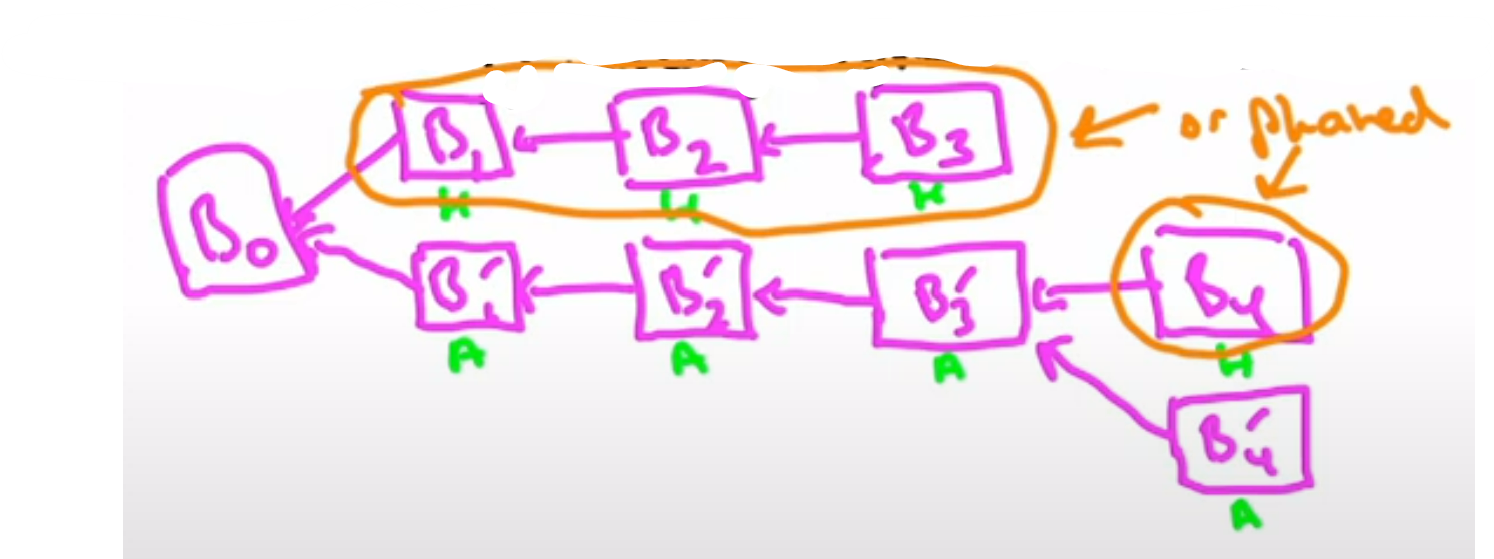
\includegraphics[scale = 0.5]{figures/f41.png}
    \caption{The example of strategy 2}
    \label{fig:mesh1}
\end{figure}\\

\noindent
\textbf{Conclusion of Strategy 2: }
As Node $A$'s alternative chain($A$-blocks) grows, it will eventually catch up and overtake the longest chain($H$-blocks) in terms of block height. This means that the longest chain will switch to Node $A$'s chain, as it is no longer. Hence, Node $A$'s chain becomes the new longest chain, and all block rewards will belong to Node $A$. When this happens, all honestly produced blocks ($B_1$, $B_2$, $B_3$, etc.) are orphaned, meaning they are no longer part of the longest chain. Instead, the longest chain now comprises only blocks produced by Node $A$.\\

\noindent
\textbf{Profit Maximization:} Node $A$'s strategy of deviating from honest behavior and orphaning honest blocks allows it to maximize its share of the block rewards. By having control over the majority of the hash rate, Node A can ensure its chain grows faster and replaces the longest chain.\\
The example above demonstrates how Node $A$, with more than 50\% of the hash rate, can successfully deviate from the protocol to maximize its block rewards by orphaning honestly produced blocks. This strategy allows Node $A$ to claim 100\% of the block rewards, which is more profitable than following the protocol obediently.\\
Note that this strategy is specific to the extreme case where Node $A$ controls more than half of the hash rate. In the next part, we will explore a variant where Node $A$ has less than 50\% hash rate and how the strategy might be tweaked to still boost Node $A$'s share of the block rewards.


\section{Selfish Mining (Worst-Case Tiebreaking}
Now, we will explore the concept of deviating from the longest chain consensus protocol and its implications on node rewards. The key takeaway is that in general, deviating from this protocol can boost the rewards of a node. We will discuss examples and strategies to demonstrate this phenomenon.

\subsection{Background}
In the previous section, we examined a scenario where a large node with more than half of the hash rate deviated from the longest chain consensus protocol, leading to several issues. Now, we will focus on a current assumption of worst-case tie-breaking by honest nodes. Under this assumption, the size of the node, big or small, will not affect its profitability to deviate from the longest chain consensus. The deviations we will discuss are often referred to as "selfish mining," where nodes prioritize profit maximization over protocol obedience.

\subsection{Selfish Mining and its History}
Selfish mining is a concept that was introduced in the field of blockchain game theory. It was first formulated by Ayal and Sirira and was disseminated in 2013, followed by formal publication in 2014. At that time, Bitcoin was the dominant blockchain network, and Nakamoto consensus was the prevailing consensus protocol.\\

The term "selfish mining" refers to a behavior exhibited by certain nodes in the blockchain network. Instead of strictly adhering to the consensus protocol and validating transactions honestly, selfish mining nodes prioritize profit maximization. They strategically deviate from the standard longest chain consensus protocol to increase their share of block rewards.\\

Ayal and Sirira's work focused specifically on Nakamoto consensus, which is the underlying consensus mechanism used in Bitcoin. Under Nakamoto consensus, blocks are produced through a proof-of-work process, and nodes compete to find the solution to a cryptographic puzzle. The node that successfully solves the puzzle gets to create the next block and is rewarded with newly minted coins and transaction fees.\\

In their research, Ayal and Sirira explored various strategies that a selfish mining node could adopt to maximize its rewards. By exploiting certain weaknesses in the consensus protocol, a selfish mining node could potentially gain an advantage over other nodes and increase its share of block rewards.\\

It's worth noting that the concept of selfish mining was a significant development in the academic sphere. The research paper on selfish mining by Alan Sharir gained widespread attention and citations, making it one of the most referenced papers in the blockchain research community.\\

Over time, the term "selfish mining" has evolved beyond its original narrow meaning. While initially specific to Nakamoto consensus and profit-motivated deviations from honest behavior, it is now used in a broader sense. Today, "selfish mining" may refer to any behavior by block producers that deviates from the intended behavior of the protocol with the goal of increasing their revenue. This broader definition includes actions like increasing transaction fees or manipulating the application layer to maximize profits.\\

In conclusion, selfish mining, as introduced by Ayal and Sirira, is a significant concept in blockchain game theory, particularly in the context of Nakamoto consensus. It has sparked extensive research and discussions within the academic community, shedding light on the complexities of blockchain incentives and the behavior of rational actors within the network.\\

Now, we're going to discuss the main subject:\\
Let node $A$ have $\alpha < \frac{1}{2}$ fraction of overall hash rate(All other nodes are honest).
\subsection{Strategy: Orphaning Blocks}

Let's delve into the strategy nodes use to increase their rewards. We'll consider a scenario where a node, denoted as Node $A$, has a hash rate $\alpha$ less than one-half. The two main ingredients of this strategy are as follows:\\
\noindent
\textbf{1. Orphaning Honestly Produced Blocks}\\
Node $A$ aims to have its blocks included in the longest chain while minimizing the number of honestly produced blocks on the chain. Unlike the previous section with 51\% hash rate, Node $A$ can't orphan all honestly produced blocks, but it still seeks to orphan the most recent ones.\\
\noindent
\textbf{2. Delaying Block Announcements}\\
Node $A$ takes advantage of the ability to delay block announcements. If Node $A$ produces blocks that outpace the honestly produced blocks, it will only announce these blocks on a need-to-know basis, ensuring that honest nodes waste their efforts on the non-longest chain.\\

\subsubsection*{Example of the Strategy (Figure 10.2)}

Let's illustrate the strategy with an example:\\
\noindent
\textbf{Step 1:} We start with the Genesis block $B_0$.\\
\noindent
\textbf{Step 2:} The next block is produced by an honest node, denoted as $B_1$.\\
Explanation: In the blockchain, new blocks are added to a chain, starting from the Genesis block. Block $B_1$ is the first block after the Genesis block, and it is honestly produced by one of the nodes following the protocol.\\
\noindent
\textbf{Step 3:} Node $A$ tries to extend the Genesis block to create an alternative block $B'_1$.\\
Explanation: Node $A$, with a hash rate $\alpha$ less than one-half, aims to increase its share of block rewards. It tries to produce an alternative block $B'_1$ that extends the Genesis block $B_0$. This is done to compete with block $B_1$ honestly produced by another node.\\
\noindent
\textbf{Step 4:} If Node $A$ successfully produces $B'_{1}$, $B_1$ gets orphaned.\\
Explanation: If Node $A$ is successful in producing $B'_1$ and announces it to the network, the honest nodes will have a tie between two blocks, $B_1$ and $B'_1$, as botH-blocks extend the same predecessor (Genesis block). In this case, the adversarial tie-breaking mechanism allows Node $A$ to extend $B'_1$, and $B_1$ becomes an orphaned block.\\
\noindent
\textbf{Step 5:} The next block is produced by an honest node, denoted as $B_2$, extending $B_1$.\\
Explanation: The honest nodes keep following the protocol, and the next block $B_2$ is produced, extending $B_1$.\\
\noindent
\textbf{Step 6:} Node $A$ concedes $B_1$ and tries to extend $B_1$ to create $B'_{2}$.\\
Explanation: Node $A$ concedes that it cannot orphan all honestly produced blocks. Instead, it focuses on the most recent ones. Here, Node A tries to extend block $B_1$ by producing $B'_2$. This is done to compete with block $B_2$ honestly produced by another node.\\
\noindent
\textbf{Step 7:} If Node $A$ successfully produces $B'_{2}$, $B_2$ gets orphaned.\\
Explanation: Similar to Step 4, if Node $A$ successfully produces $B'_2$ and announces it, it creates a tie between $B_2$ and $B'_2$. As Node $A$ has a lower hash rate, the adversarial tie-breaking mechanism favors the block $B'_2$ produced by Node $A$, leading to the orphaning of $B_2$.\\
\noindent
\textbf{Step 8:} Node $A$ keeps the existence of $B'_{3}$ private and lets honest nodes extend $B_2$.\\
Explanation: Node $A$ continues the strategy of delaying block announcements. It produces a block $B'_3$ but does not immediately announce it to the network. Instead, it keeps it private. Meanwhile, the honest nodes continue extending block $B_2$.\\
\noindent
\textbf{Step 9:} Once an honest node produces a block $B_3$ extending $B_2$, Node $A$ announces $B'_{3}$.\\
Explanation: Node $A$ waits until an honest node produces a block $B_3$ that extends $B_2$. At this point, Node $A$ announces its private block $B'_3$. This is done strategically to trick the honest nodes into extending the non-longest chain.\\
\noindent
\textbf{Step 10:} Honest nodes extend $B'_{3}$, orphaning $B_3$.\\
Explanation: The honest nodes, unaware of the existence of $B'_3$ due to Node A's delay in announcing it, keep extending block $B'_3$. As a result, $B_3$ becomes an orphaned block.\\
\begin{figure}[h]
    \centering
    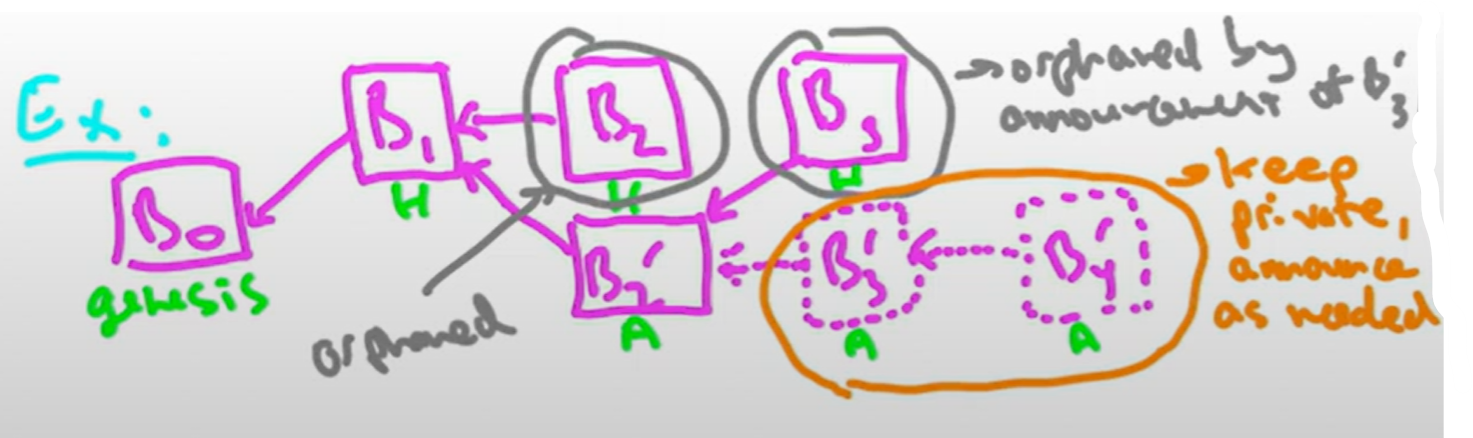
\includegraphics[scale = 0.5]{figures/f42.png}
    \caption{The example of strategy for the case of $\alpha < \frac{1}{2}$}
    \label{fig:mesh1}
\end{figure}\\

Node $A$'s strategy for increasing its share of block rewards involves two cases, depending on whether Node $A$ is ahead in block production or if the honest nodes are ahead. Let $h$ denote the maximum height of any block produced thus far. (Remember that by block height we just mean the number of steps since Genesis)

\subsection*{Case 1: Node $A$ is Ahead}
In this case, Node $A$ is in an advantageous position, meaning it has already produced a block at the highest block height (denoted as $h$) among all the blocks that have been created. The strategy for Node $A$ is straightforward:
\noindent
\textbf{Step 1:} Node $A$ extends its own block at height $h$ to create an alternative block (denoted as $B'_{h}$).\\
\noindent
\textbf{Step 2:} Node $A$ delays announcing block $B'_h$, keeping it private for now.\\
\noindent
\textbf{Step 3:} If Node $A$ successfully produces another block at height $h$ (denoted as $B"_{h}$), it also keeps this block private.\\
\noindent
\textbf{Step 4:} Node $A$ waits until an honest node produces a block at height $h$ (denoted as $B_h$).\\
\noindent
\textbf{Step 5:} Once an honest node announces $B_h$, Node $A$ immediately announces its previously private block $B'_h$.\\
\noindent
\textbf{Step 6:} Honest nodes, unaware of Node $A$'s private block, start extending the longest chain with $B_h$ as the new tip. Node $A$, however, already has its private block $B'_h$, so it extends its own chain.\\
\noindent
\textbf{Step 7:} Honest nodes and Node $A$ will now compete to extend their respective chains from heights $h$ and $h'$. Node $A$ aims to win this competition, which will result in orphaning $B_h$ and keeping its own block $B'_h$ as part of the longest chain.\\

\subsection*{Case 2: Honest Nodes are Ahead}

In this case, the highest block height (denoted as $h$) among all the blocks produced so far was created by an honest node, not Node $A$. The strategy for Node $A$ in this situation is as follows:\\
\noindent
\textbf{Step 1:} Node A tries to produce a block at height $h$, extending the same block as the honest node (denoted as $B'_h$).\\
\noindent
\textbf{Step 2:} Node A delays announcing block $B'_h$, keeping it private.\\
\noindent
\textbf{Step 3:} If Node A successfully produces $B'_h$, it waits until an honest node creates a block at height $h$ (denoted as $B_h$).\\
\noindent
\textbf{Step 4:} Node A immediately announces its private block $B'_h$ once an honest node announces $B_h$.\\
\noindent
\textbf{Step 5:} Honest nodes will be unaware of Node $A$'s private block and extend the longest chain from height $h$ using $B_h$ as the new tip. However, Node $A$'s private block $B'_h$ is already longer than any honestly produced block from height $h$.\\
\noindent
\textbf{Step 6:} Honest nodes and Node A will compete to extend their respective chains from heights $h$ and $h'$. Node $A$ aims to win this competition, which will result in orphaning $B_h$ and keeping its own block $B'_h$ as part of the longest chain.\\

\noindent
\textbf{Throughout:} Announce an A-block of height $h$ as soon as there's an H-block at height $h$.

\subsection{Analysis}
Sure, here are the full notes in LaTeX form:
The analysis focuses on a sequence of $N$ consecutive rounds, where $N$ is a reasonably large number, to study the fraction of blocks produced by Node $A$ on the longest chain.

\subsubsection*{Step 1: Block Creation Expectations}
Considering the $N$ blocks, we expect an $\alpha$ fraction to be produced by Node $A$ (A-Blocks) and a $(1 - \alpha)$ fraction to be produced by honest nodes(H-blocks). This expectation relies on the random oracle assumption for block creation probability.

\subsubsection*{Step 2: All Node A-Blocks on Longest Chain}
Every block created by Node $A$ is guaranteed to be on the longest chain at the time of announcement. Thus, all Node A-blocks stay on the longest chain forever.

\subsubsection*{Step 3: Orphaning Honest Blocks}
For every block created by Node $A$, an honestly produced block is orphaned due to adversarial tie-breaking. Thus, the number of orphaned honest blocks is the same as the number of Node $A$ blocks.\\

\noindent
\textbf{Calculations:}\\
Let's calculate the fraction of Node $A$'s blocks on the longest chain compared to the total blocks.\\
\noindent
\# of A-blocks: The total number of Node $A$ blocks is approximately $\alpha N$, and all of them are on the longest chain.\\
\noindent
\# of H-blocks: The total number of honest blocks is approximately $(1 - \alpha)N$, and approximately $\alpha N$ of them are orphaned, leaving $(1 - 2\alpha)N$ honest blocks on the longest chain.\\

\newpage
\noindent
Fraction of Node $A$ Blocks: The fraction of Node $A$'s blocks on the longest chain is:
$$
\frac{\alpha N}{(1 - \alpha)N} = \frac{\alpha}{1 - \alpha}
$$

For any positive value of $\alpha$, the fraction $\frac{\alpha}{1 - \alpha}$ is larger than $\alpha$, meaning selfish mining boosts Node $A$'s rewards, regardless of its hash rate. Even for small values of $\alpha$, this strategy provides a significant increase in block rewards. The analysis also highlights a connection between selfish mining and the chain quality guarantees from Chapter 8. The strategy's impact will be discussed further in the upcoming sections.

\section{Selfish Mining (Best-Case Tiebreaking)}
In this section, we will examine the third and final version of the argument known as selfish mining, which involves deviating from the intended behavior and longest chain consensus. The focus will be on how this deviation can boost the share of block rewards earned by a node running the protocol.

\subsection{Relaxing Assumptions}
We will start by relaxing the assumption that we made in previous chapters, where we allowed the deviating node (node $A$) to control how honest nodes break ties among competing longest chains. This assumption was inherited from chapter eight, where we were studying the consistency and liveness properties of longest chain consensus. However, for analyzing selfish mining in a profit-maximizing node, we need to assume the opposite: the tie-breaking is not under the control of node $A$, and honest nodes will extend the longest chain with an honestly produced block at its tip.

\textbf{Impact of Assumption:}\\
Making this new assumption will make the analysis more challenging and complex than before. The strategy for the deviating node becomes more intricate, and the analysis becomes harder. The result will be weaker than before, indicating that deviating from longest chain consensus will be beneficial only for nodes possessing a substantial fraction of the hash rate (around 33\% or more) but not for smaller nodes.

To illustrate the consequence of this assumption, we provide a simple example with a fork in the blockchain. Let's break down the explanation:
\begin{itemize}
    \item \textbf{The Scenario:} There is a fork in the blockchain with two tips, $B_1$ and $B_2$, which have the same predecessor block B. $B_1$ is produced by an honest node (H-block), and $B'_1$ is produced by node $A$ (A-block).
    \item \textbf{Previous Scenario:} In the previous section, the assumption was that node $A$ had control over tie-breaking, so it could determine that all honest nodes would extend the A block $B'_1$. In that case, node $A$ would be sure that its block $B'_1$ would end up in the longest chain.
    \item \textbf{Current Scenario:} However, in this video, the assumption is that honest nodes decide to extend the chain with an honestly produced block at its tip (H block) instead of the deviating node $A$ block (A-block). Now, node $A$ is not sure that its block $B'_1$ will end up in the longest chain.
    \item\textbf{Risk in Orphaning H-blocks:} Node $A$ may try to orphan the H block $B_1$ by creating a competing block at the same height, which it successfully does ($B'_1$). However, for $B_1$ to be orphaned, node $A$ needs to create a second block ($B'_2$) extending $B'_1$, and only then will honest nodes switch to extending the chain of A-blocks. Until this happens, honest nodes will keep extending the chain of H-blocks.
    \item \textbf{Consequences of Failure:} If an honest node creates a block ($B_2$) before node $A$ produces $B'_2$, node $A$ will be even further behind in chain length, and its attempts to orphan H-blocks will be increasingly challenging.
    \item \textbf{Complicated Analysis:} Due to these complex forces, the analysis becomes more intricate. The speaker mentions that the benefit of orphaning H-blocks by node $A$ is uncertain and depends on the hash rate (Alpha) possessed by node $A$.
    \item \textbf{Impact on Deviation:} The uncertainty in the cost-benefit analysis indicates that whether deviating from the consensus protocol is profitable or not depends on the hash rate $\alpha$. For sufficiently large nodes, deviating from the protocol may be a good idea, but for smaller nodes, it might not be beneficial.
\end{itemize}
Overall, the impact of this assumption on tie-breaking introduces new challenges and complexities in the analysis, making it harder to determine the profitability of the deviation for different hash rates possessed by the deviating node. 

\begin{figure}[h]
    \centering
    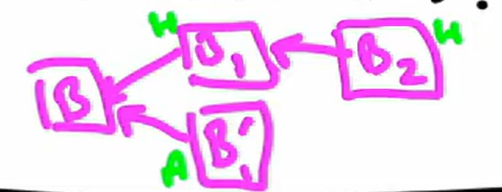
\includegraphics[scale = 0.5]{figures/f43.png}
    \caption{Consequence of the assumption}
    \label{fig:mesh1}
\end{figure}\\

\textbf{Modeling the Strategy: }We will parameterize the analysis by the fraction of the hash rate possessed by the deviating node (node $A$), denoted as $\alpha$. For $\alpha < \frac{1}{2}$, we will consider the case where all other nodes (1 - $\alpha$ fraction) follow the protocol honestly without profit maximization considerations. The goal is to understand if honesty is contagious in Nakamoto consensus or if a deviation leads to a Nash equilibrium.

\subsection{Four Cases of Strategy}
We will now describe the four cases of the strategy for node $A$ based on different scenarios. We're going to keep track of two different block Heights $h_p$ that's going to be the highest height
the maximum height of every block that's been announced to everybody of course every honestly produced block has been
announced to everybody because that's what honest nodes do node $A$ will be selectively releasing announcements of
blocks so all of the publicly announced blocks the highest height one among those is going to be $h_p$ node $A$ may
also have some blocks that are secret that only it knows about and if there are any such blocks $h_s$ is going to
denote the highest height among all of them.\\
Remember that the height of a block in a blockchain is the number of hops that you need to get back to Genesis or
equivalently it's the length of the chain that ends at that block. So
the end of the longest chain is going to be exactly the block with the maximum height. For example, $h_p$ is the maximum height of any publicly announced block
from the perspective of the honest nodes who know only about the public announce blocks; they think that the longest chain
is currently whichever one ends at the Block that has height $h_p$. Node $A$
meanwhile may know about blocks at even higher Heights if node $A$ ever chooses to release all those blocks that will create a new longest chain.

\subsubsection{Case 1: No Secret Blocks ($h_p > h_s$)}
In this case, Node $A$ doesn't have any secret blocks, meaning all its blocks are publicly announced and known to everyone. Node $A$'s goal is to maximize its share of the block rewards by getting as many of its blocks as possible into the longest chain, where block rewards are earned. The honest nodes, constituting the majority of the network (1 - $\alpha$) fraction of the hash rate), are also following the protocol honestly and are trying to extend the longest chain, which is currently at height $h_p$.

Node $A$ recognizes that its current position in the blockchain is not ahead of the honest nodes' longest chain. So, it decides to extend the publicly announced longest chain, trying to produce a new block, let's say $B_{4}'$, which would extend the current longest chain with a block of its own. In this way, Node $A$ hopes to get its own block rewards and increase its share of the pie.

Meanwhile, the honest nodes continue extending the longest chain, aiming to produce an honestly produced block, say $B_{4}$, at height $h_p +1$. This honest block will compete with Node $A$'s secretly created block $B_{4}'$.\\

\begin{figure}[h]
    \centering
    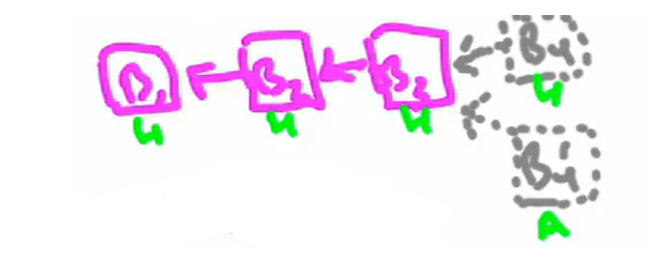
\includegraphics[scale = 0.5]{figures/f44.png}
    \caption{Case 1}
    \label{fig:mesh1}
\end{figure}\\

\noindent
\textbf{Outcome 1: Node A's Success}\\
With probability $\alpha$, Node $A$ succeeds in being the first one to produce a new block ($B_{4}'$) extending the longest chain. At this point, Node $A$ keeps this newly created block secret and continues with its strategy.\\
\noindent
\textbf{Outcome 2: Honest Node's Success}\\
With probability $1-\alpha$, one of the honest nodes succeeds in producing an honestly generated block $B_{4}$ at height $h_p +1$. Now, Node $A$'s secretly created block $B_{4}'$ is not part of the longest chain, and the honest nodes continue extending their chain.\\

In either case, the situation remains in Case 1, and Node $A$ continues trying to extend the longest chain, aiming to gain more control over the blockchain.

\subsubsection{Case 2: Secret Block Created ($h_s = h_p + 1$)}
In this case, Node $A$ successfully creates a secret block $B_{4}'$, which extends the longest chain with a new block at height $h_p +1$. Node $A$'s privately held chain now has a height of $h_p +1$, and it has a lead of one block over the publicly known longest chain maintained by the honest nodes.\\

Node $A$ now faces a strategic decision: whether to continue keeping its newly created block $B_{4}'$ secret or to publicly announce it to the network. If it chooses to announce it, the honest nodes will realize that a new longest chain exists, starting from block $B_{4}'$. In this situation, the honest nodes will switch to extending the chain with Node $A$'s blocks, as they always choose the longest chain with the latest honestly produced block at the tip.\\

\begin{figure}[h]
    \centering
    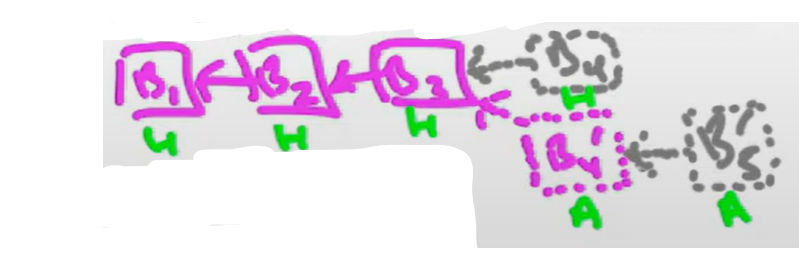
\includegraphics[scale = 0.5]{figures/f45.png}
    \caption{Case 2}
    \label{fig:mesh1}
\end{figure}\\
\noindent
\textbf{Outcome 1: Node A Continues with Secret Block}\\
With probability $\alpha$, Node $A$ decides to keep its newly created block $B_{4}'$ secret and tries to extend it further to increase its lead over the publicly known longest chain.\\
\noindent
\textbf{Outcome 2: Node A Announces Secret Block}\\
With probability $1-\alpha$, Node $A$ chooses to announce its new block $B_{4}'$ to the network. This action changes the dynamics of the blockchain, leading to the network recognizing a new longest chain with Node A's blocks at its tip.\\

At this point, the situation moves to Case 4, where Node $A$ has a secret block lead over the publicly known longest chain maintained by the honest nodes.
It is important to note that Case 2 is reached only when Node $A$ successfully creates a secret block that extends the longest chain, giving it a one-block lead. If it fails to do so, it will remain in Case 1 and continue extending the publicly known longest chain.

\subsubsection{Case 3: Extending Private Chain($h_s = h_p$)}

In Case 3, Node $A$ is in a position where it already has a secret block $B_{4}'$ (B4 Prime) that it created back in Case 1. Node $A$ is not willing to give up on this secret chain and is determined to extend it further. Meanwhile, the honest nodes are following their usual strategy of extending the end of the longest chain they know about.\\
\begin{figure}[h]
    \centering
    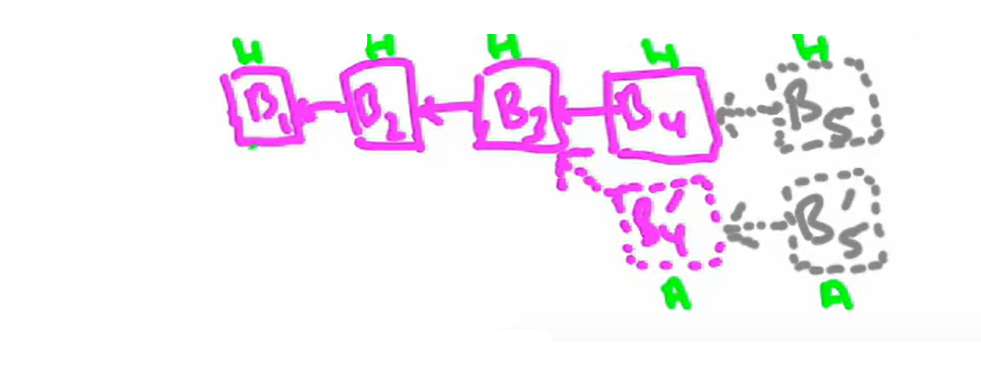
\includegraphics[scale = 0.5]{figures/f46.png}
    \caption{Case 3}
    \label{fig:mesh1}
\end{figure}\\
\noindent
\textbf{Outcome 1: Node A's Success}\\
If Node $A$ successfully creates another secret block, say $B_{5}'$ (B5 Prime), before the honest nodes are able to produce a block $B_{5}$, then Node $A$ gains a lead of two blocks over the honest chain. In this situation, Node $A$ announces both its secret blocks ($B_{4}'$ and $B_{5}'$).\\

By announcing both secret blocks, Node $A$ effectively declares victory, making this new chain the universally recognized longest chain. The honest nodes were trying to create a block $B_{5}$, but they did not do it in time. Now, with the announcement of $B_{4}'$ and $B_{5}'$, these blocks are guaranteed membership in the longest chain. The honest nodes have no choice but to recognize this new chain and continue extending it.

This scenario is a win for Node $A$, as it managed to extend its secret chain and get its private blocks into the longest chain.\\

\noindent
\textbf{Outcome 2: Honest Node's Success}\\
If the honest nodes successfully produce a block $B_{5}$ before Node $A$ creates $B_{5}'$, then Node $A$'s lead over the honest chain shrinks to just one block. In this case, Node $A$ realizes that its chances of winning the race to extend the longest chain are diminishing. It decides to abandon its secret chain and return to Case 1, where it tries to extend the honest nodes' longest chain.

Node $A$ accepts the fact that its secret block $B_{4}'$ got orphaned and it no longer has an advantage over the honest nodes. It acknowledges the honest nodes' new longest chain, which includes block $B_{5}$, and decides to move on.

\subsubsection{Case 4: Large Secret Chain Lead ($h_s \geq h_p +2$}
In Case 4, Node $A$ has managed to build a private chain with a lead of two or more blocks over the publicly known longest chain maintained by the honest nodes.\\
\begin{figure}[h]
    \centering
    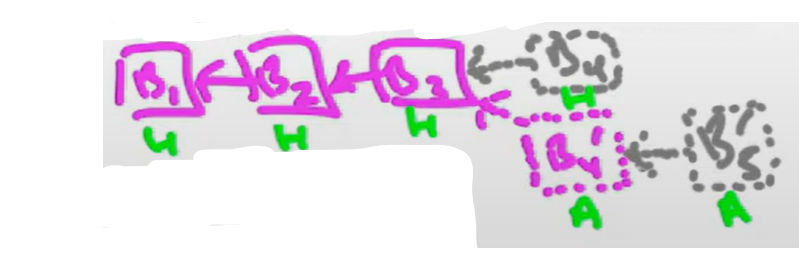
\includegraphics[scale = 0.5]{figures/f45.png}
    \caption{Case 4}
    \label{fig:mesh1}
\end{figure}\\
\noindent
\textbf{Outcome 1: Node A Keeps Extending Secret Chain}\\
If Node $A$ continues to succeed in extending its secret chain, creating block $B_{6}'$ (B6 Prime), and maintains a lead of two or more blocks over the honest chain, it will keep extending its private chain.

Node $A$ recognizes that its secret chain is significantly ahead of the honest chain, and as long as it can maintain this lead, it is in a favorable position to continue extending its private chain.\\

\noindent
\textbf{Outcome 2: Honest Node's Success}\\
If the honest nodes manage to produce a block that closes the gap to just one block between Node $A$'s secret chain and the honest chain, Node $A$ faces a dilemma. It realizes that its advantage is diminishing rapidly, and there is a risk of its private blocks getting orphaned.

In this situation, Node $A$ decides not to take any further risks and immediately announces all its secret blocks (e.g., $B_{4}'$, $B_{5}'$, $B_{6}'$) to the network. This action ensures that all of Node $A$'s secret blocks become part of the longest chain and guarantees their inclusion.

By announcing all its secret blocks at once, Node $A$ ensures that the deepest of its secret blocks ($B_{6}'$) becomes the new universally recognized longest chain. The honest nodes have no choice but to follow this new chain.

The announcement of multiple secret blocks might lead to the orphaning of some of the honestly produced blocks, but Node $A$ accepts this trade-off to ensure its secret blocks are securely in the longest chain.\\

\noindent
\textbf{Outcome 3: Honest Node's Success (Lead Shrinks to One)}\\
If the honest nodes manage to produce a block that further reduces the gap to just one block between Node $A$'s secret chain and the honest chain, Node $A$ takes immediate action to secure its secret blocks.

With a lead of only one block, Node $A$ realizes that its position is becoming risky. It decides not to take any further chances and announces all its secret blocks (e.g., $B_{4}'$, $B_{5}'$, $B_{6}'$) to the network. This ensures the inclusion of all its secret blocks into the longest chain.

In this scenario, Node $A$ announces three secret blocks at once, which guarantees their membership in the longest chain. These secret blocks orphan some of the honestly produced blocks, but Node $A$ prioritizes securing its secret blocks and their inclusion in the longest chain.

\subsubsection{Summary}
The mining strategy employed by Node $A$ is a complex interplay of different factors. It involves balancing the benefits of orphaning honestly produced blocks with the risk of having its secret blocks orphaned. Whether the strategy is a good idea or not depends on the hash rates of Node $A$ and the honest nodes.\\

In Case 1, Node $A$ follows the standard protocol and tries to extend the publicly known longest chain. It competes with the honest nodes to get its blocks into the chain and maximize its share of block rewards. However, this straightforward approach does not provide Node $A$ with any special advantage.\\

In Case 2, Node $A$ successfully creates a secret block that extends the longest chain, giving it a one-block lead. At this point, Node $A$ faces a critical decision: whether to keep its newly created block secret or to announce it to the network. If Node $A$ keeps it secret, it can continue extending its lead and possibly gain more control over the blockchain. If it announces the secret block, the honest nodes will recognize a new longest chain, starting from Node $A$'s block. Node $A$'s advantage, in this case, depends on whether it can continue creating secret blocks to maintain its lead.\\

Case 3 represents a riskier situation for Node $A$. Here, Node $A$ already has one secret block, but the honest nodes have produced a block that narrows the gap to one block between Node $A$'s secret chain and the honest chain. Node $A$ attempts to create another secret block to maintain its lead, but if the honest nodes produce a block before it does, Node $A$ will abandon its secret chain and go back to Case 1.\\

In Case 4, Node $A$ enjoys a significant lead, with two or more secret blocks ahead of the publicly known chain. This is the most favorable situation for Node $A$, as it can keep extending its secret chain with lower risk. However, if the honest nodes manage to close the gap to one block, Node $A$ will immediately announce all its secret blocks to ensure they get into the longest chain. This is a defensive move to avoid losing the advantage gained from having a large lead.\\

Analyzing the effectiveness of Node $A$'s strategy requires non-trivial mathematical analysis. The outcome depends on the relative hash rates of Node $A$ and the honest nodes. If Node $A$ has a significant hash rate advantage, its strategy may lead to more of its blocks being included in the longest chain, potentially increasing its share of block rewards. On the other hand, if Node $A$'s hash rate is relatively small compared to the honest nodes, its strategy may result in more of its blocks getting orphaned, leading to lower rewards.\\

Overall, the mining strategy employed by Node $A$ demonstrates the complexities and challenges of deviating from the standard protocol in a blockchain network. It illustrates the importance of considering various factors, such as hash rates, block creation speed, and the risk of block orphaning, when devising a mining strategy. Mathematical analysis is necessary to determine the optimal strategy in different scenarios and to understand the potential impact on the overall network dynamics.

\section{Markov Chain Analysis}
Markov Chains are mathematical models used to describe random processes that exhibit the Markov property. The Markov property states that the future state of the system depends only on the current state and is independent of the past states. In other words, the future evolution of the system is memoryless and is determined solely by the current state.\\
In this section, we will analyze the strategy for node $A$ in Nakamoto consensus. The strategy involves a tricky tug-of-war between two competing forces. The node may decide to deviate from obediently following the longest chain consensus, and the decision depends on the amount of hash rate that node A possesses. We will explore different cases and transitions using a Markov chain analysis.

\subsection{Markov Chains and Transition Probabilities}
Markov chains are useful in modeling random processes. In this context, we can represent the different states of the strategy with vertices and the probabilities of transitioning between states with directed edges.

A Markov chain has two main components: the set of states (vertices) and the transition probabilities (directed edges). We will use non-negative integers to label the states, representing how big a lead node A has in its secret chain relative to the publicly known chain.

\section{States and Transitions}
Let's define the states for our Markov chain:
\begin{itemize}
    \item State 0: No lead at all (corresponds to case one).\\
    This state represents the situation where node $A$ does not have any lead in its secret chain compared to the publicly known chain. In this case, node A simply tries to extend the end of the publicly known longest chain. There is no advantage for node $A$ in this state.
    \item State 1: A lead of one (corresponds to case two).\\
    This state represents the scenario where node $A$ has a lead of one in its secret chain over the publicly known chain. Node $A$ has successfully extended the longest chain one block ahead. In this state, node $A$ will keep the newly created block private and not reveal it to the network immediately.
    \item State $f$: Fork state (corresponds to case three).\\
    This state occurs when there is a tie between one of the blocks in node $A$'s secret chain and the publicly known chain. Node $A$ has succeeded in extending the longest chain, but an honest node has also produced a block at the same height. This results in a fork in the blockchain.
    \item State $i$: Lead of $i$ (corresponds to case four, where $i \geq 2$).\\
    This state represents the situation where node $A$ has a lead of $i$ in its secret chain over the publicly known chain. Node $A$ has successfully extended the longest chain $i$ blocks ahead. In this state, node $A$ will keep the $i$ newly created blocks private.
\end{itemize}

We will now explore the transitions between these states based on the strategy cases.

\subsection{Strategy Cases and Transition Probabilities}
\subsubsection{Case One}
Corresponds to State 0. Node $A$ just tries to extend the end of the publicly known longest chain.
\begin{itemize}
    \item If node $A$ succeeds, it keeps the block private and transitions to State 1 with probability $\alpha$.
    \item If node $A$ fails (an honest node succeeds), it remains in State 0 with probability $1 - \alpha$. This means there is a $(1 - \alpha)$ chance that node $A$ will still have no lead over the publicly known chain in the next step.
\end{itemize}

\begin{tikzpicture}[->,>=stealth',shorten >=1pt,auto,node distance=2.5cm,semithick]
    \tikzstyle{every state}=[draw=black,text=black,minimum size=1cm]

    \node[state] (0) {0};
    \node[state] (1) [right of=0] {1};

    \path (0) edge node {$\alpha$} (1)
          (0) edge [loop above] node {$1-\alpha$} (0);
\end{tikzpicture}

\subsubsection{Case Two}
Corresponds to State 1. Node $A$ has a lead of one in its secret chain over the publicly known chain.
\begin{itemize}
    \item If node $A$ succeeds in extending the longest chain, it gains a lead of two and transitions to State 2 with probability $\alpha$. This means there is an $\alpha$ chance that node $A$ will have a lead of two in its secret chain over the publicly known chain in the next step.
    \item If node $A$ fails (an honest node extends the longest chain), it transitions to State $f$ (fork state) with probability $1 - \alpha$. This means there is a $(1 - \alpha)$ chance that node $A$ will encounter a fork in the blockchain in the next step.
\end{itemize}

\begin{tikzpicture}[->,>=stealth',shorten >=1pt,auto,node distance=2.5cm,semithick]
    \tikzstyle{every state}=[draw=black,text=black,minimum size=1cm]

    \node[state] (1) {1};
    \node[state] (2) [right of=1] {2};
    \node[state] (f) [below of=1] {$f$};

    \path (1) edge node {$\alpha$} (2)
          (1) edge node [left] {$1-\alpha$} (f);
\end{tikzpicture}

\subsubsection{Case Three}
Corresponds to State $f$ (fork state). Node $A$ has a tie between one of its private blocks and the publicly known block.
\begin{itemize}
    \item If node A succeeds in extending its secret chain (breaking the tie), it transitions back to State 0 with probability $\alpha$. This means there is an $\alpha$ chance that node A will restart its strategy with no lead over the publicly known chain.
    \item If node A fails (an honest node extends the longest chain), it also transitions back to State 0 with probability $1 - \alpha$. This means there is a $(1 - \alpha)$ chance that node A will restart its strategy with no lead over the publicly known chain.
\end{itemize}

\begin{tikzpicture}[->,>=stealth',shorten >=1pt,auto,node distance=2.5cm,semithick]
    \tikzstyle{every state}=[draw=black,text=black,minimum size=1cm]

    \node[state] (f) {$f$};
    \node[state] (0) [right of=f] {0};

    \path (f) edge [bend left] node {$\alpha$} (0)
          (f) edge [loop below] node {$1-\alpha$} (f);
\end{tikzpicture}

\subsubsection{Case Four}
Corresponds to State $i$ (lead of $i$). Node $A$ has a lead of $i$ in its secret chain over the publicly known chain.
\begin{itemize}
    \item If node $A$ succeeds in extending its secret chain, it increases its lead by one and transitions to State $i+1$ with probability $\alpha$. This means there is an $\alpha$ chance that node A will have a lead of $(i+1)$ in its secret chain over the publicly known chain in the next step.
    \item If node $A$ fails (an honest node extends the longest chain), it decreases its lead by one and transitions to State $i-1$ with probability $1 - \alpha$. This means there is a $(1 - \alpha)$ chance that node A will have a lead of $(i-1)$ in its secret chain over the publicly known chain in the next step.
\end{itemize}

\begin{tikzpicture}[->,>=stealth',shorten >=1pt,auto,node distance=2.5cm,semithick]
    \tikzstyle{every state}=[draw=black,text=black,minimum size=1cm]

    \node[state] (i-1) {$i-1$};
    \node[state] (i) [right of=i-1] {$i$};
    \node[state] (i+1) [right of=i] {$i+1$};

    \path (i-1) edge [bend right] node [below] {$1-\alpha$} (i)
          (i) edge node {$\alpha$} (i+1);
\end{tikzpicture}

Note: For $i=2, 3, 4, \ldots$, the pattern continues with transitions between states $i-1$ and $i+1$.\\

\noindent\textbf{Transition Probabilities:}\\
\begin{enumerate}
    \item From State 0 to State 1:
    \begin{itemize}
        \item Probability of success (creating a block): $\alpha$
        \item Probability of failure (an honest node creates a block): $1 - \alpha$
    \end{itemize}
    \item From State 1 to State 2:
    \begin{itemize}
        \item Probability of success (creating a block): $\alpha$
        \item Probability of failure (an honest node creates a block): $1 - \alpha$
    \end{itemize}
    \item From State 1 to State $f$(fork state):
    \begin{itemize}
        \item Probability of success (creating a block): $1 - \alpha$ (Node A loses the race)
        \item Probability of failure (an honest node creates a block): $\alpha$ (Node A wins the race)
    \end{itemize}
    \item From State $f$ to State 0:
    \begin{itemize}
        \item Probability of success (creating a block): $1 - \alpha$ (Node A loses the race)
        \item Probability of failure (an honest node creates a block): $\alpha$ (Node A wins the race)
    \end{itemize}
    \item From State $f$ to State $f$:
    \begin{itemize}
        \item Probability of success (creating a block): $1 - \alpha$ (Node $A$ loses the race)
        \item Probability of failure (an honest node creates a block): $\alpha$ (Node $A$ wins the race)
    \end{itemize}
    \item From State $i$ to State $i+1$:
    \begin{itemize}
        \item Probability of success (creating a block): $1 - \alpha$ (Node $A$ loses the race)
        \item Probability of failure (an honest node creates a block): $\alpha$ (Node $A$ wins the race)
    \end{itemize}
    \item From State $i$ to State $i-1$:
    \begin{itemize}
        \item Probability of success (creating a block): $1 - \alpha$ (Node $A$ loses the race)
        \item Probability of failure (an honest node creates a block): $\alpha$ (Node $A$ wins the race)
    \end{itemize}
\end{enumerate}

The following Figure 10.8 demonstrates the transition probability of all cases, all together:\\
\begin{figure}[h]
    \centering
    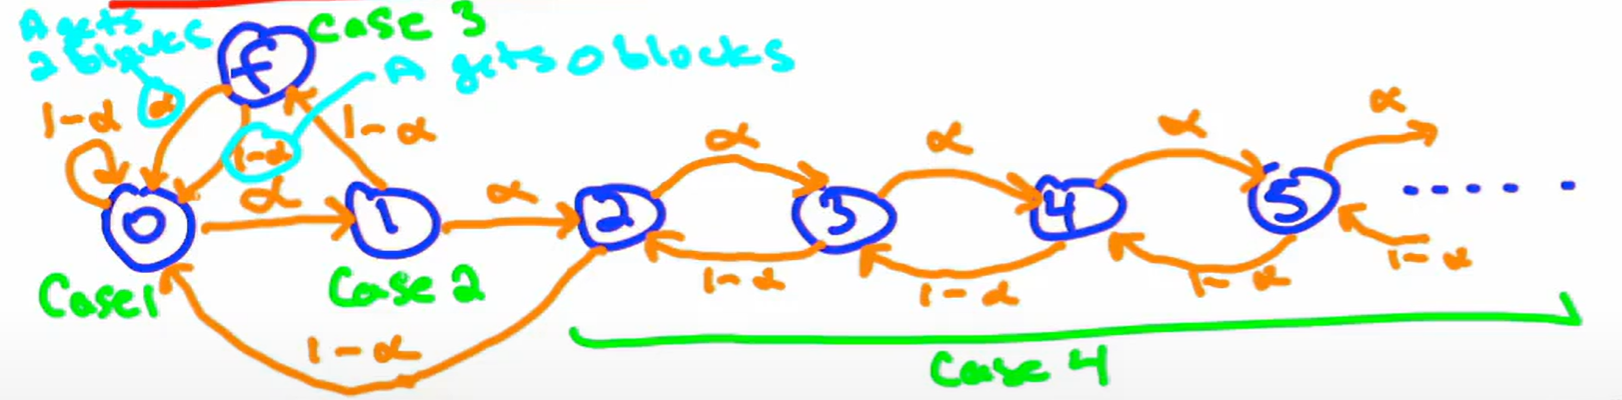
\includegraphics[scale = 0.5]{figures/f48.png}
    \caption{Transition Probabilities}
    \label{fig:mesh1}
\end{figure}\\

Remember that $\alpha$ represents the probability that node $A$ wins the race in creating the next block, and $1 - \alpha$ represents the probability that an honest node wins the race in creating the next block.\\

These states and transition probabilities are essential in understanding how the proposed strategy behaves in different scenarios and help in analyzing its long-term implications in Nakamoto consensus. By analyzing the strategy using Markov chains, we can determine the probabilities of transitioning between different states and understand the potential outcomes for node A. This analysis helps us assess the effectiveness of the strategy and the block rewards that node A can expect in different scenarios.

\subsection{Stationary Distributions}
A stationary distribution in a Markov chain represents the equilibrium or long-run frequency of each state. In our case, it corresponds to the relative amount of time that the system spends in each state. The stationary probability of State $i$ is denoted by $\pi_i$, which is also considered the long-run frequency of spending time in that state.

\noindent
\textbf{Computing Stationary Distribution:}\\
To compute the stationary distribution for the specific Markov chain being discussed, let's consider the limit as a parameter $T$ approaches infinity. The idea is to observe the system's behavior over an increasingly large number of transitions to understand the long-term probabilities of being in each state.\\
Let's delve deeper into the computation process:\\
The stationary probability of each state is denoted by $\pi_i$, where $i$ represents the state in the Markov chain. For this specific Markov chain with two states (State 0 and State 1), we need to find the values of $\pi_0$ and $\pi_1$.

$$
\pi_i = \lim_{{T \to \infty}} \frac{{\text{Number of visits to State } i}}{{T}}
$$

This means that to find $\pi_i$, we need to consider the number of times the system visits State $i$ during $T$ transitions and take the limit of this ratio as $T$ approaches infinity.

Note that the numerator of the ratio involves the count of consecutive transitions that land in State $i$ (the number of visits to State $i$). The denominator $T$ represents the total number of transitions or steps taken in the system.

The numerator, i.e., the number of visits to State $i$, is a random variable. It depends on how the transitions occur, and therefore, it may vary each time the experiment is conducted. However, although the numerator is a random variable, we can consider its expected value. This involves finding the average number of visits to State $i$ over the long run.

The expectation of the number of visits to State $i$ can be computed as:

$$
\text{Expected visits to State } i = \lim_{{T \to \infty}} \frac{{\text{Total visits to State } i}}{{T}}
$$

Now, we can rewrite the stationary probability $\pi_i$ in terms of the expected visits to State $i$:

$$
\pi_i = \lim_{{T \to \infty}} \frac{{\text{Total visits to State } i}}{{T}} = \lim_{{T \to \infty}} \frac{{\text{Expected visits to State } i}}{{T}}
$$

As $T$ approaches infinity, the denominator $T$ becomes very large, making the fraction infinitesimally small. As a result, the stationary probability $\pi_i$ becomes the limit of the expected number of visits to State $i$ divided by an infinitely large number:

$$
\pi_i = \lim_{{T \to \infty}} \frac{{\text{Expected visits to State } i}}{{T}}
$$

It's important to note that the stationary distribution is independent of the initial state from which the system starts. This means that no matter where the system begins (State 0 or State 1), the long-run frequencies of being in each state will converge to the same values. There are closed-form formulas available for computing the stationary probabilities $\pi_0$ and $\pi_1$.


\subsection{Strategy and Block Counting}
We now explore a specific strategy involving the Markov chain described earlier. The strategy is designed to decide which block to extend in a blockchain system. The key objective is to understand how good this strategy is compared to the standard approach of following the longest chain.

\subsubsection{Markov Chain and Strategy}
The Markov chain in question consists of two states: State 0 and State 1. The transition probabilities between these states are denoted by $\alpha$ and $1 - \alpha$, respectively. The strategy is defined by different cases of block competition, which we refer to as cases one through four.\\

In case one, the strategy begins with an honest node extending the longest chain. On the other hand, in case two, node A creates a block but doesn't immediately add it to the longest chain. Instead, it keeps the block private, awaiting a possible lead in the future. If an honest node creates the next block in case two, the block created by node A in case one will be orphaned. Thus, it is too early to count this block toward node A's total.\\

Case three involves a more complex situation. Here, there is a competition between node A's private chain and the honest chain, which have the same height. Whichever chain gets extended first becomes part of the longest chain, and the other block becomes orphaned. In this case, node A is guaranteed to get two new blocks on the longest chain if it wins the competition. Likewise, if the honest nodes find the next block, they are also guaranteed to have two new blocks on the longest chain.\\

In case four, the situation is more straightforward. Every block created by node A is certain to end up on the longest chain, and every block created by the honest nodes will be orphaned. Therefore, transitioning from any state $i$ to state $i+1$ will always add one block to node A's total.

\subsubsection{Block Counting Exercise}
To evaluate the strategy's effectiveness, we conduct a block counting exercise for each transition in the Markov chain. This exercise helps determine how many blocks produced by node A and how many blocks produced by honest nodes end up on the longest chain.\\

\noindent
\textbf{Case One (State 0)}\\
In case one, an honest node extends the longest chain. This block can be confidently counted as it will always be part of the longest chain.\\

\noindent
\textbf{Case Two (State 1)}\\
In case two, node In case two, node $A$ creates a block but doesn't immediately add it to the longest chain. Instead, it keeps the block private, waiting for the next block to be created. If an honest node creates the next block, the block created by node A will be orphaned. Thus, it is not yet appropriate to count this block toward node A's total.\\

\noindent
\textbf{Case Three (State $f$)}\\
Case three involves a competition between node $A$'s private chain and the honest chain. Whichever chain gets extended becomes part of the longest chain. If node $A$ wins the competition, it is guaranteed to have two new blocks on the longest chain. Similarly, if the honest nodes win the competition, they are also guaranteed to have two new blocks on the longest chain.\\

\noindent
\textbf{Case Four (State 2, 3, 4, etc.)}\\
In case four, every block created by node $A$ is certain to end up on the longest chain. Conversely, every block created by the honest nodes will be orphaned. Therefore, every transition from state $i$ to state $i+1$ adds one block to node A's total.\\

By conducting the block counting exercise for each transition, we identify the number of blocks that will be added to node $A$'s total on the longest chain for each scenario. This analysis lays the foundation for evaluating the effectiveness of the strategy compared to the traditional approach of following the longest chain consensus.

\subsection{Evaluating the Strategy}
We can use the stationary distribution of the Markov chain to evaluate the strategy's performance. To do this, we need to compute the stationary probabilities $\pi_i$ for each state. As stated, the stationary distribution represents the long-run frequency with which the system spends time in each state.

\subsubsection{Expression for Honest Nodes' Blocks}
The number of blocks produced by honest nodes that end up on the longest chain is given by:
$$
\text{Honest nodes' blocks} = \pi_0 \cdot (1 - \alpha) + \pi_f \cdot (1 - \alpha) \cdot 2$$
The term $\pi_0 \cdot (1 - \alpha)$ represents the probability that an honest node creates a block in State 0 (case one) and adds it to the longest chain. This happens with a probability of $(1 - \alpha)$ when the system is in State 0 (case one), and $\pi_0$ is the stationary probability of being in State 0.
The term $\pi_f \cdot (1 - \alpha) \cdot 2$ accounts for the probability that an honest node extends the longest chain when the system is in State $F$ (case three). In this case, two new blocks are guaranteed to be added to the longest chain (one for the publicly announced block and one for the private block of node A). $\pi_f$ is the stationary probability of being in State $F$, and $(1 - \alpha)$ is the probability that an honest node finds the next block.

\subsubsection{Expression for Node $A$'s Blocks}
The number of blocks produced by node A that end up on the longest chain is given by:
$$
\text{Node A's blocks} = \sum_{i=1}^{\infty} \pi_i \cdot \alpha + \pi_f \cdot \alpha \cdot 2
$$
The term $\sum_{i=1}^{\infty} \pi_i \cdot \alpha$ represents the probability that node A creates a block in State $i$ (case two) and successfully extends its private chain to State $i+1$. This is the case for all states from 1 to infinity. The summation considers all possible states in which node A produces a block, weighted by their stationary probabilities $\pi_i$.
The term $\pi_f \cdot \alpha \cdot 2$ accounts for the probability that node A extends the public chain from State $F$ (case three) and adds its private block and the publicly announced block to the longest chain. The stationary probability $\pi_f$ is used, and $\alpha$ represents the probability of node A finding the next block.\\

By evaluating the expressions for the number of blocks produced by node A and honest nodes, we can determine how good the strategy is compared to following the standard longest chain consensus. By comparing the results, we can identify the specific scenarios where this strategy outperforms the traditional approach.

\subsection{Final Calculations}
The main question is: What is the fraction of blocks on the longest chain that node $A$ will have if it follows this strategy? We compare this fraction with the standard approach of honestly following the longest chain consensus, where node $A$ would get a share of the blocks proportional to its hash rate.

\subsubsection{Computing the Stationary Distribution}
\textbf{Linear Relationships in the Stationary Distribution}\\
To compute the stationary distribution, we identify a few simple linear relationships between the stationary probabilities. These relationships are derived from the structure of the Markov chain.
\begin{itemize}
    \item \textbf{Condition 1:} $\pi_1 = \alpha \cdot \pi_0$

    This condition represents the relationship between $\pi_0$ and $\pi_1$. Here, $\pi_0$ is the probability of the system being in State 0, which corresponds to the state where node $A$ has an empty private chain and the public longest chain is one block ahead. $\pi_1$ is the probability of the system being in State 1, where node $A$ has successfully mined the next block on its private chain and has caught up to the public longest chain.
    
    The equation $\pi_1 = \alpha \cdot \pi_0$ indicates that the probability of transitioning from State 0 to State 1 is given by $\alpha$, which is the probability that node $A$ successfully finds the next block. In other words, if node $A$ has an empty private chain (State 0), the chance of it mining the next block and reaching State 1 is $\alpha$. This makes intuitive sense as $\alpha$ represents node A's hash rate relative to the total hash rate of the network.
    \item \textbf{Condition 2:} $\pi_f = (1 - \alpha) \cdot \pi_1$

    Condition 2 establishes a relationship between $\pi_1$ and $\pi_f$. In this context, $\pi_f$ represents the probability of the system being in State $f$, which denotes the state where the public longest chain is $F$ blocks ahead of node $A$'s private chain. Here, $f$ can be any positive integer.
    
    The equation $\pi_f = (1 - \alpha) \cdot \pi_1$ means that the probability of transitioning from State 1 to State $F$ is given by $(1 - \alpha)$. In other words, if node $A$ has successfully mined the next block on its private chain (State 1), the chance of the public longest chain being $f$ blocks ahead (State $f$) is $(1 - \alpha)$. This reflects the probability that an honest node mines the next block and extends the public longest chain while node $A$ is working on its private chain.

    \item \textbf{Condition 3:} $\pi_i \cdot \alpha = \pi_{i+1} \cdot (1 - \alpha)$ for all positive integers $i$

    Condition 3 provides a general relationship between $\pi_i$ and $\pi_{i+1}$ for all positive integers $i$. Here, $\pi_i$ represents the probability of the system being in State $i$, and $\pi_{i+1}$ represents the probability of the system being in the next state, State $i+1$.
    
    The equation $\pi_i \cdot \alpha = \pi_{i+1} \cdot (1 - \alpha)$ states that the probability of transitioning from State $i$ to State $i+1$ is given by $\alpha$, while the probability of transitioning from State $i+1$ back to State $i$ is given by $(1 - \alpha)$. This captures the dynamics of the Markov chain, where at each step, node $A$ either mines a block and advances its private chain with probability $\alpha$, or an honest node mines a block and extends the public longest chain with probability $(1 - \alpha)$.

\end{itemize}
By combining these linear relationships, we can see how all the stationary probabilities $\pi_i$ can be expressed in terms of $\pi_0$. The sum of all stationary probabilities should be equal to 1, which allows us to solve for $\pi_0$ explicitly. Once $\pi_0$ is determined, all other stationary probabilities can be obtained using the linear relationships.               

\subsection{Ratio of Block Rewards}
Once we have the stationary probabilities, we can compute the ratio of block rewards obtained by node $A$ when following the selfish mining strategy to the rewards it would get by following the longest chain consensus.

The final ratio is a function of $\alpha$, representing the fraction of blocks that node $A$ successfully mines, and is given by:
$$ \text{Ratio} = \frac{4\alpha^3 - 9\alpha^2 + 4\alpha}{\alpha^3 - 2\alpha^2 - \alpha + 1} $$
This ratio serves as a measure of how much more block rewards node $A$ can gain through the selfish mining strategy compared to honest mining. If the ratio is greater than 1, it indicates that selfish mining is more profitable for node $A$, while a ratio less than 1 means that honest mining is more advantageous.\\

The analysis of selfish mining shows that if node $A$ has a hash rate greater than one-third of the network's total hash rate, it is incentivized to deviate from the honest longest chain consensus. By employing the selfish mining strategy, node $A$ can obtain a larger share of block rewards than it would get by following the standard approach.\\

While the specific strategy analyzed in this section is not optimal, it is still close to the optimal strategy. There are more sophisticated strategies that can provide even better rewards when node A's hash rate is slightly below one-third. However, when node $A$'s hash rate is less than one-third, it is in its best interest to follow the longest chain consensus honestly.\\

Selfish mining analysis provides valuable insights into the incentives and behaviors of miners in a blockchain network and has significant implications for the security and stability of the network.

\section{Discussion}
In this final part of chapter 10, we will review what we have learned from the analysis of selfish mining, deviations from honest behavior, and Nakamoto consensus. We will also discuss the practical implications of this analysis.\\

\noindent
\textbf{Selfish Mining and Nash Equilibrium}
In this chapter, we started by emphasizing the crucial aspect of introducing a native cryptocurrency into a blockchain. It enables nodes to receive rewards for creating blocks. However, it is not always the case that incentivizing nodes to follow the longest chain consensus protocol results in a Nash equilibrium, where all nodes behave honestly.\\

Three different scenarios were presented to illustrate how selfish mining strategies can provide an incentive for nodes to deviate from honest behavior. The first scenario involves a node with 51\% of the hash rate, which can guarantee 100\% of the block rewards by consistently orphaning honestly produced blocks. The second scenario considers nodes with less than 50\% of the hash rate but with the ability to influence how honest nodes resolve competing longest chains. In this case, a slightly more complicated strategy boosts the deviating node's share of the block rewards regardless of its hash rate. The third scenario is the most complex, where a node neither has 51\% of the hash rate nor control over communication networks. Despite this, it can still benefit from selfish mining deviations, but only if it possesses more than a third of the total hash rate.\\

\noindent
\textbf{Academic Literature Influence}
This chapter also acknowledges the influential paper by Ayal and Sirer, published in 2014, which has sparked a vast array of follow-up works. These subsequent studies explore various aspects of selfish mining and deviations in different blockchain protocols, such as Ethereum 1.0 and various proof-of-stake designs. The academic community's exploration into these areas has been instrumental in understanding the implications of these strategies.

\noindent
\textbf{Practice and Implications}
Despite the theoretical analysis suggesting potential deviations, there is no evidence of nodes using these strategies in the 13 years of Bitcoin's existence.

Possible explanations for this lack of observed deviations include:
\begin{enumerate}
    \item Capital Requirements: It is challenging to accumulate enough hash rate to execute the selfish mining strategy effectively, which might require a substantial investment in specialized hardware.
    \item Delayed Payoff: The benefits of the deviation would take a long time to materialize due to the difficulty adjustment mechanism in Nakamoto consensus. This delayed payoff increases the risk and reduces the incentive for potential attackers.
    \item Potential Price Crash: Some argue that public knowledge of an attack might lead to a drop in the price of the native cryptocurrency, resulting in the attacker losing wealth. However, this argument is not entirely convincing since prices are not always as sensitive to such attacks as believed.
\end{enumerate}
Despite not being observed in practice, we should underscore the importance of the game-theoretic analysis in blockchain protocols. It demonstrates that in the context of cryptocurrencies and native incentives, the behavior of nodes cannot be solely classified as honest or Byzantine, and a more nuanced analysis is required.\\

\noindent
\textbf{Conclusion}\\
Understanding game theory and incentive structures in blockchain protocols is crucial. The analysis presented in this chapter emphasizes the need for a nuanced approach to node behavior, beyond simple classifications of honest or Byzantine. While selfish mining strategies may not have been observed in practice so far, it is essential to remain vigilant and thoroughly assess the incentive mechanisms within blockchain systems. Future considerations should be given to revenue streams, including block rewards, transaction fees, and value from transactions. The upcoming chapter on Ethereum's EIP 1559 will delve further into transaction fee mechanism design. Stay tuned!

A creates a block but doesn't immediately add it to the longest chain. Instead, it keeps the block private, waiting for the next block to be created. If an honest node creates the next block, the block created by node A will be orphaned. Thus, it is not yet appropriate to count this block toward node A's total.\\

\noindent
\textbf{Case Three (State $f$)}\\
Case three involves a competition between node A's private chain and the honest chain. Whichever chain gets extended becomes part of the longest chain. If node A wins the competition, it is guaranteed to have two new blocks on the longest chain. Similarly, if the honest nodes win the competition, they are also guaranteed to have two new blocks on the longest chain.\\

\noindent
\textbf{Case Four (State 2, 3, 4, etc.)}\\
In case four, every block created by node A is certain to end up on the longest chain. Conversely, every block created by the honest nodes will be orphaned. Therefore, every transition from state $i$ to state $i+1$ adds one block to node A's total.\\

By conducting the block counting exercise for each transition, we identify the number of blocks that will be added to node A's total on the longest chain for each scenario. This analysis lays the foundation for evaluating the effectiveness of the strategy compared to the traditional approach of following the longest chain consensus.

\subsection{Evaluating the Strategy}
We can use the stationary distribution of the Markov chain to evaluate the strategy's performance. To do this, we need to compute the stationary probabilities $\pi_i$ for each state. As stated, the stationary distribution represents the long-run frequency with which the system spends time in each state.

\subsubsection{Expression for Honest Nodes' Blocks}
The number of blocks produced by honest nodes that end up on the longest chain is given by:
$$
\text{Honest nodes' blocks} = \pi_0 \cdot (1 - \alpha) + \pi_f \cdot (1 - \alpha) \cdot 2$$
The term $\pi_0 \cdot (1 - \alpha)$ represents the probability that an honest node creates a block in State 0 (case one) and adds it to the longest chain. This happens with a probability of $(1 - \alpha)$ when the system is in State 0 (case one), and $\pi_0$ is the stationary probability of being in State 0.
The term $\pi_f \cdot (1 - \alpha) \cdot 2$ accounts for the probability that an honest node extends the longest chain when the system is in State $F$ (case three). In this case, two new blocks are guaranteed to be added to the longest chain (one for the publicly announced block and one for the private block of node A). $\pi_f$ is the stationary probability of being in State $F$, and $(1 - \alpha)$ is the probability that an honest node finds the next block.

\subsubsection{Expression for Node A's Blocks}
The number of blocks produced by node A that end up on the longest chain is given by:
$$
\text{Node A's blocks} = \sum_{i=1}^{\infty} \pi_i \cdot \alpha + \pi_f \cdot \alpha \cdot 2
$$
The term $\sum_{i=1}^{\infty} \pi_i \cdot \alpha$ represents the probability that node A creates a block in State $i$ (case two) and successfully extends its private chain to State $i+1$. This is the case for all states from 1 to infinity. The summation considers all possible states in which node A produces a block, weighted by their stationary probabilities $\pi_i$.
The term $\pi_f \cdot \alpha \cdot 2$ accounts for the probability that node A extends the public chain from State $F$ (case three) and adds its private block and the publicly announced block to the longest chain. The stationary probability $\pi_f$ is used, and $\alpha$ represents the probability of node A finding the next block.\\

By evaluating the expressions for the number of blocks produced by node A and honest nodes, we can determine how good the strategy is compared to following the standard longest chain consensus. By comparing the results, we can identify the specific scenarios where this strategy outperforms the traditional approach.

\subsection{Final Calculations}
The main question is: What is the fraction of blocks on the longest chain that node A will have if it follows this strategy? We compare this fraction with the standard approach of honestly following the longest chain consensus, where node A would get a share of the blocks proportional to its hash rate.

\subsubsection{Computing the Stationary Distribution}
\textbf{Linear Relationships in the Stationary Distribution}\\
To compute the stationary distribution, we identify a few simple linear relationships between the stationary probabilities. These relationships are derived from the structure of the Markov chain.
\begin{itemize}
    \item \textbf{Condition 1:} $\pi_1 = \alpha \cdot \pi_0$

    This condition represents the relationship between $\pi_0$ and $\pi_1$. Here, $\pi_0$ is the probability of the system being in State 0, which corresponds to the state where node A has an empty private chain and the public longest chain is one block ahead. $\pi_1$ is the probability of the system being in State 1, where node A has successfully mined the next block on its private chain and has caught up to the public longest chain.
    
    The equation $\pi_1 = \alpha \cdot \pi_0$ indicates that the probability of transitioning from State 0 to State 1 is given by $\alpha$, which is the probability that node A successfully finds the next block. In other words, if node A has an empty private chain (State 0), the chance of it mining the next block and reaching State 1 is $\alpha$. This makes intuitive sense as $\alpha$ represents node A's hash rate relative to the total hash rate of the network.
    \item \textbf{Condition 2:} $\pi_f = (1 - \alpha) \cdot \pi_1$

    Condition 2 establishes a relationship between $\pi_1$ and $\pi_f$. In this context, $\pi_f$ represents the probability of the system being in State $f$, which denotes the state where the public longest chain is $F$ blocks ahead of node A's private chain. Here, $f$ can be any positive integer.
    
    The equation $\pi_f = (1 - \alpha) \cdot \pi_1$ means that the probability of transitioning from State 1 to State $F$ is given by $(1 - \alpha)$. In other words, if node A has successfully mined the next block on its private chain (State 1), the chance of the public longest chain being $f$ blocks ahead (State $f$) is $(1 - \alpha)$. This reflects the probability that an honest node mines the next block and extends the public longest chain while node A is working on its private chain.

    \item \textbf{Condition 3:} $\pi_i \cdot \alpha = \pi_{i+1} \cdot (1 - \alpha)$ for all positive integers $i$

    Condition 3 provides a general relationship between $\pi_i$ and $\pi_{i+1}$ for all positive integers $i$. Here, $\pi_i$ represents the probability of the system being in State $i$, and $\pi_{i+1}$ represents the probability of the system being in the next state, State $i+1$.
    
    The equation $\pi_i \cdot \alpha = \pi_{i+1} \cdot (1 - \alpha)$ states that the probability of transitioning from State $i$ to State $i+1$ is given by $\alpha$, while the probability of transitioning from State $i+1$ back to State $i$ is given by $(1 - \alpha)$. This captures the dynamics of the Markov chain, where at each step, node A either mines a block and advances its private chain with probability $\alpha$, or an honest node mines a block and extends the public longest chain with probability $(1 - \alpha)$.

\end{itemize}
By combining these linear relationships, we can see how all the stationary probabilities $\pi_i$ can be expressed in terms of $\pi_0$. The sum of all stationary probabilities should be equal to 1, which allows us to solve for $\pi_0$ explicitly. Once $\pi_0$ is determined, all other stationary probabilities can be obtained using the linear relationships.               

\subsection{Ratio of Block Rewards}
Once we have the stationary probabilities, we can compute the ratio of block rewards obtained by node A when following the selfish mining strategy to the rewards it would get by following the longest chain consensus.

The final ratio is a function of $\alpha$, representing the fraction of blocks that node A successfully mines, and is given by:
$$ \text{Ratio} = \frac{4\alpha^3 - 9\alpha^2 + 4\alpha}{\alpha^3 - 2\alpha^2 - \alpha + 1} $$
This ratio serves as a measure of how much more block rewards node A can gain through the selfish mining strategy compared to honest mining. If the ratio is greater than 1, it indicates that selfish mining is more profitable for node A, while a ratio less than 1 means that honest mining is more advantageous.\\

The analysis of selfish mining shows that if node A has a hash rate greater than one-third of the network's total hash rate, it is incentivized to deviate from the honest longest chain consensus. By employing the selfish mining strategy, node A can obtain a larger share of block rewards than it would get by following the standard approach.\\

While the specific strategy analyzed in this section is not optimal, it is still close to the optimal strategy. There are more sophisticated strategies that can provide even better rewards when node A's hash rate is slightly below one-third. However, when node A's hash rate is less than one-third, it is in its best interest to follow the longest chain consensus honestly.\\

Selfish mining analysis provides valuable insights into the incentives and behaviors of miners in a blockchain network and has significant implications for the security and stability of the network.

\section{Discussion}
In this final part of chapter 10, we will review what we have learned from the analysis of selfish mining, deviations from honest behavior, and Nakamoto consensus. We will also discuss the practical implications of this analysis.\\

\noindent
\textbf{Selfish Mining and Nash Equilibrium}
In this chapter we started by emphasizing the crucial aspect of introducing a native cryptocurrency into a blockchain. It enables nodes to receive rewards for creating blocks. However, it is not always the case that incentivizing nodes to follow the longest chain consensus protocol results in a Nash equilibrium, where all nodes behave honestly.\\

Three different scenarios were presented to illustrate how selfish mining strategies can provide an incentive for nodes to deviate from honest behavior. The first scenario involves a node with 51\% of the hash rate, which can guarantee 100\% of the block rewards by consistently orphaning honestly produced blocks. The second scenario considers nodes with less than 50\% of the hash rate, but with the ability to influence how honest nodes resolve competing longest chains. In this case, a slightly more complicated strategy boosts the deviating node's share of the block rewards regardless of its hash rate. The third scenario is the most complex, where a node neither has 51\% of the hash rate nor control over communication networks. Despite this, it can still benefit from selfish mining deviations, but only if it possesses more than a third of the total hash rate.\\

\noindent
\textbf{Academic Literature Influence}
This chapter also acknowledges the influential paper by Ayal and Sirer, published in 2014, which has sparked a vast array of follow-up works. These subsequent studies explore various aspects of selfish mining and deviations in different blockchain protocols, such as Ethereum 1.0 and various proof-of-stake designs. The academic community's exploration into these areas has been instrumental in understanding the implications of these strategies.

\noindent
\textbf{Practice and Implications}
Despite the theoretical analysis suggesting potential deviations, there is no evidence of nodes using these strategies in the 13 years of Bitcoin's existence.

Possible explanations for this lack of observed deviations include:
\begin{enumerate}
    \item Capital Requirements: It is challenging to accumulate enough hash rate to execute the selfish mining strategy effectively, which might require a substantial investment in specialized hardware.
    \item Delayed Payoff: The benefits of the deviation would take a long time to materialize due to the difficulty adjustment mechanism in Nakamoto consensus. This delayed payoff increases the risk and reduces the incentive for potential attackers.
    \item Potential Price Crash: Some argue that public knowledge of an attack might lead to a drop in the price of the native cryptocurrency, resulting in the attacker losing wealth. However, this argument is not entirely convincing since prices are not always as sensitive to such attacks as believed.
\end{enumerate}
Despite not being observed in practice, we should underscore the importance of the game-theoretic analysis in blockchain protocols. It demonstrates that in the context of cryptocurrencies and native incentives, the behavior of nodes cannot be solely classified as honest or Byzantine, and a more nuanced analysis is required.\\

\noindent
\textbf{Conclusion}\\
Understanding game theory and incentive structures in blockchain protocols is crucial. The analysis presented in this chapter emphasizes the need for a nuanced approach to node behavior, beyond simple classifications of honest or Byzantine. While selfish mining strategies may not have been observed in practice so far, it is essential to remain vigilant and thoroughly assess the incentive mechanisms within blockchain systems. Future considerations should be given to revenue streams, including block rewards, transaction fees, and value from transactions. The upcoming chapter on Ethereum's EIP 1559 will delve further into transaction fee mechanism design. Stay tuned!









